\documentclass[slidestop,usepdftitle=false,10pt]{beamer}
\usepackage[accumulated]{beamerseminar}
\usepackage[english]{babel}
%\usepackage{beamertexpower}
\usepackage{multicol}
\usetheme{Antibes}
\usepackage{adjustbox}
%\usepackage{beamerthemeshadow}
\usepackage[utf8]{inputenc}
%\usepackage[spanish]{babel}
\usepackage{amsmath}
\usepackage{amsfonts}
\usepackage{amssymb}
\usepackage{graphicx}
\usepackage{mathtools,amssymb}
%\usepackage{subfigure}
%\usepackage{subfig}
\usepackage{caption}
%\usepackage{subcaption}
\usepackage{bm}
\usepackage{booktabs}
\usepackage{optidef}
\usepackage{amsthm}
\usepackage{comment}
\usepackage{pgfplots}
\usepackage{soul}
\usepackage{mathrsfs}
\usepackage[ruled]{algorithm2e}
\usepackage{xspace}
\usepackage{ulem}
\usepackage{multirow}
\usepackage{bigstrut}
% \usepackage{booktabs}
\usepackage{url}
%\usepackage{enumitem}
%\usepackage{algorithm}
%\usepackage{algpseudocode}


%\usetheme[height=0mm]{Rochester}
%\usepackage[spanish]{babel}
%\usepackage[utf8]{inputenc}
%\input adefin.tex
%\beamertemplatenavigationsymbolsempty
%\beamersetaveragebackground{white!90!red}
%**********************************************************
\newtheorem{defn}{Definition}[section]
\newtheorem{ej}{Example}[section]
\newtheorem{ejs}{Examples}[section]
\newtheorem{prop}{Proposition}
\newtheorem{nota}{Notation}[section]
\newtheorem{thm}{Theorem}[section]
\newtheorem{cor}{Corollary}[section]
\newtheorem{rem}{Remark}[section]
\newtheorem{lem}{Lemma}[section]

\def \Proof{\noindent{\underline {Proof:}}}
\def\fra#1#2{\frac{ #1}{ #2}}
\renewcommand*{\baselinestretch}{1}

\def\fra#1#2{\frac{ #1}{ #2}}
%\def\fra#1#2{\frac{\displaystyle #1}{\displaystyle #2}}
%\renewcommand*{\baselinestretch}{1}

\def\fra#1#2{\frac{\displaystyle #1}{\displaystyle #2}}

%\newcommand{\fra}[2]{\displaystyle{\frac{#1}{#2}}}
\DeclareMathOperator*{\argmin}{arg\,min}

\newcommand{\KMPHN}{{\sf{H-KMPHN}}}
\newcommand{\KMPN}{{\sf{H-KMPN}\xspace }}
\newcommand{\SPPN}{{\sf{H-SPPN}\xspace }}
\newcommand{\TSPN}{{\sf{H-TSPN}\xspace }}
\newcommand{\TSPVN}{{\sf{H-TSPVN}\xspace }}
\newcommand{\B}{{\mathcal B}}
\newcommand{\VB}{{V^{}_{\mathcal B}}}
\newcommand{\EB}{{E^{}_{\mathcal B}}}
\newcommand{\EBint}{{E^{int}_{\mathcal B}}}
\newcommand{\VS}{{V^{}_{\mathcal S}}}
\newcommand{\ES}{{E^{}_{\mathcal S}}}
\newcommand{\VT}{{V^{}_{\mathcal T}}}
\newcommand{\ET}{{E^{}_{\mathcal T}}}
\newcommand{\VX}{{V^{}_X}}
\newcommand{\EX}{{E^{}_X}}
\newcommand{\VN}{{V^{}_{\mathcal N}}}
\newcommand{\EN}{{E^{}_{\mathcal N}}}
\newcommand{\EST}{{E^{}_{\mathcal S\mathcal T}}}
\newcommand{\GSPP}{{G_{\text{SPP}}}}
\newcommand{\VSPP}{{V_{\text{SPP}}}}
\newcommand{\ESPP}{{E_{\text{SPP}}}}
\newcommand{\GTSP}{{G_{\text{TSP}}}}
\newcommand{\VTSP}{{V_{\text{TSP}}}}
\newcommand{\ETSP}{{E_{\text{TSP}}}}
\newcommand{\GKMPHN}{{G_{\text{KMPHN}}}}
\newcommand{\VKMPHN}{{V_{\text{KMPHN}}}}
\newcommand{\EKMPHN}{{E_{\text{KMPHN}}}}
\newcommand{\GKMPN}{{G_{\text{KMPN}}}}
\newcommand{\VKMPN}{{V_{\text{KMPN}}}}
\newcommand{\EKMPN}{{E_{\text{KMPN}}}}
\newcommand{\VSS}{{V^*_S}}
\newcommand{\ESS}{{E^*_S}}
\newcommand{\VTS}{{V^*_T}}
\newcommand{\ETS}{{E^*_T}}
\newcommand{\VNS}{{V^*_{\mathcal N}}}
\newcommand{\ENS}{{E^*_{\mathcal N}}}
\newcommand{\GSPPS}{{G^{*}_{\text{SPP}}}}
\newcommand{\VSPPS}{{V^{*}_{\text{SPP}}}}
\newcommand{\ESPPS}{{E^{*}_{\text{SPP}}}}
\newcommand{\GTSPS}{{G^{*}_{\text{TSP}}}}
\newcommand{\VTSPS}{{V^{*}_{\text{TSP}}}}
\newcommand{\ETSPS}{{E^{*}_{\text{TSP}}}}

\newtheorem{remark}{Remark}
\newtheorem{notation}{Notation}

%\newtheorem{prop}{Proposition}

\definecolor{armygreen}{rgb}{0.19, 0.53, 0.43}
\definecolor{atomictangerine}{rgb}{1.0, 0.6, 0.4}
\newcommand{\JP}[1]{{\color{armygreen}#1}}
\newcommand{\CV}[1]{{\color{red}#1}}
\newcommand{\segment}[2]{\overline{#1#2}}
\newcommand{\determinant}[3]{\det({#1|#2#3})}

\setbeamertemplate{enumerate subitem}{\alph{enumii}}
	
%%%%%%%%%%%%%%%%%
\definecolor{31}{rgb}{.3,.5,.2}
\definecolor{13}{rgb}{.1,.6,.3}
% CHANGED: Moved \title and \author outside of slide
\title[Combining neighbourhoods with barriers]{\textsc{The Hampered Traveling Salesman Problem with Neighbourhoods}}
\author[IWOLOCA-2023]{Carlos Valverde Mart\'in}
%\newline
\institute{
	\begin{center}
		\date{}
		\text{XII International Workshop on Locational Analysis and Related Problems 2023}
	\end{center}
	\begin{center}
		\textcolor{blue}{Joint work with Justo Puerto}
	\end{center}
	\begin{center}
		
\includegraphics[width=0.15\textwidth]{logo.jpg}
	\end{center}
}
\date{}

\usefonttheme{professionalfonts}

\begin{document}
	\begin{frame}
		\titlepage
	\end{frame}
	%Trasparencias
	

	\section{The Hampered Traveling Salesman Problem with Neighbourhoods}
	\begin{frame}{Contents}
	    \begin{itemize}
	    	\item Problem Motivation
		    \item Problem Description
		    \item Formulation
		    \item Strengthening
		    \item Computational Experiments
		    \item Future research
%		    \item Strengthening the formulation
%		    \item Matheuristic
%		    \item Computational Experiments
%		    \item Case Study
		\end{itemize}
	\end{frame}

	\subsection{Problem Motivation}
	\begin{frame}{Problem Motivation}
		\footnotesize
		The starting point of this work is the $k$-Median Problem with Neighbourhoods (KMPN):
		\pgfplotsset{compat=1.15}
	
\usetikzlibrary{arrows}
\definecolor{ffqqqq}{rgb}{1,0,0}
\definecolor{qqwuqq}{rgb}{0,0.39215686274509803,0}
\definecolor{qqqqff}{rgb}{0,0,1}
\definecolor{ududff}{rgb}{0.30196078431372547,0.30196078431372547,1}
\begin{figure}[h!]
    \centering
    \begin{tikzpicture}[line cap=round,line join=round,>=triangle 45,x=0.1cm,y=0.1cm, scale = 0.3]
        \begin{axis}[
            x=0.1cm,y=0.1cm,
            axis lines=middle,
            xmin=-5,
            xmax=105,
            ymin=-5,
            ymax=105,
            xtick={0,10,...,100},
            ytick={0,10,...,100},]
            \draw [rotate around={0:(10,15)},line width=2pt,color=qqqqff,fill=qqqqff,fill opacity=0.25] (10,15) ellipse (0.6cm and 0.6cm);
            \draw [rotate around={0:(70,55)},line width=2pt,color=qqwuqq,fill=qqwuqq,fill opacity=0.25] (70,55) ellipse (0.4cm and 0.4cm);
            \draw [rotate around={0:(50,70)},line width=2pt,color=qqwuqq,fill=qqwuqq,fill opacity=0.25] (50,70) ellipse (0.8cm and 0.8cm);
            \draw [rotate around={0:(65,10)},line width=2pt,color=qqqqff,fill=qqqqff,fill opacity=0.25] (65,10) ellipse (0.7cm and 0.7cm);
            \draw [rotate around={0:(10,65)},line width=2pt,color=qqqqff,fill=qqqqff,fill opacity=0.25] (10,65) ellipse (0.5cm and 0.5cm);
            \draw [rotate around={0:(30,35)},line width=2pt,color=qqwuqq,fill=qqwuqq,fill opacity=0.25] (30,35) ellipse (1cm and 1cm);
            \draw [rotate around={0:(90,35)},line width=2pt,color=qqqqff,fill=qqqqff,fill opacity=0.25] (90,35) ellipse (0.6cm and 0.6cm);
            \draw [rotate around={0:(90,85)},line width=2pt,color=qqqqff,fill=qqqqff,fill opacity=0.25] (90,85) ellipse (0.6cm and 0.6cm);
            \draw [rotate around={0:(30,90)},line width=2pt,color=qqqqff,fill=qqqqff,fill opacity=0.25] (30,90) ellipse (1cm and 1cm);
        \end{axis}
    \end{tikzpicture}
\end{figure}
		\begin{itemize}
		\item $\mathcal S$: Set of neighbourhoods that describe the possible sources where a facility can be allocated. It is assumed, wlog, that one facility can be allocated to each source at most once.
		\item $\mathcal T$: Set of neighbourhoods that represent the targets that a facility must serve. It is assumed, wlog, that each target is served when it has been assigned to a facility.
		\end{itemize}
	\end{frame}
	\begin{frame}{Problem Motivation}
		\footnotesize
		Barriers that can not be crossed are taken into account in the KMPN:
		\pgfplotsset{compat=1.15}
	
\usetikzlibrary{arrows}
\definecolor{ffqqqq}{rgb}{1,0,0}
\definecolor{qqwuqq}{rgb}{0,0.39215686274509803,0}
\definecolor{qqqqff}{rgb}{0,0,1}
\definecolor{ududff}{rgb}{0.30196078431372547,0.30196078431372547,1}
\begin{figure}[h!]
    \centering
    \begin{tikzpicture}[line cap=round,line join=round,>=triangle 45,x=0.1cm,y=0.1cm, scale = 0.65]
        \begin{axis}[
            x=0.1cm,y=0.1cm,
            axis lines=middle,
            xmin=-5,
            xmax=105,
            ymin=-5,
            ymax=105,
            xtick={0,10,...,100},
            ytick={0,10,...,100},]
            \draw [rotate around={0:(10,15)},line width=2pt,color=qqqqff,fill=qqqqff,fill opacity=0.25] (10,15) ellipse (0.6cm and 0.6cm);
            \draw [rotate around={0:(70,55)},line width=2pt,color=qqwuqq,fill=qqwuqq,fill opacity=0.25] (70,55) ellipse (0.4cm and 0.4cm);
            \draw [rotate around={0:(50,70)},line width=2pt,color=qqwuqq,fill=qqwuqq,fill opacity=0.25] (50,70) ellipse (0.8cm and 0.8cm);
            \draw [rotate around={0:(65,10)},line width=2pt,color=qqqqff,fill=qqqqff,fill opacity=0.25] (65,10) ellipse (0.7cm and 0.7cm);
            \draw [rotate around={0:(10,65)},line width=2pt,color=qqqqff,fill=qqqqff,fill opacity=0.25] (10,65) ellipse (0.5cm and 0.5cm);
            \draw [rotate around={0:(30,35)},line width=2pt,color=qqwuqq,fill=qqwuqq,fill opacity=0.25] (30,35) ellipse (1cm and 1cm);
            \draw [rotate around={0:(90,35)},line width=2pt,color=qqqqff,fill=qqqqff,fill opacity=0.25] (90,35) ellipse (0.6cm and 0.6cm);
            \draw [rotate around={0:(90,85)},line width=2pt,color=qqqqff,fill=qqqqff,fill opacity=0.25] (90,85) ellipse (0.6cm and 0.6cm);
            \draw [rotate around={0:(30,90)},line width=2pt,color=qqqqff,fill=qqqqff,fill opacity=0.25] (30,90) ellipse (1cm and 1cm);
            \draw [line width=2pt,color=ffqqqq] (0,90)-- (30,60);
            \draw [line width=2pt,color=ffqqqq] (40,50)-- (10,50);
            \draw [line width=2pt,color=ffqqqq] (0,30)-- (10,40);
            \draw [line width=2pt,color=ffqqqq] (10,30)-- (30,5);
            \draw [line width=2pt,color=ffqqqq] (40,10)-- (70,40);
            \draw [line width=2pt,color=ffqqqq] (60,20)-- (100,10);
            \draw [line width=2pt,color=ffqqqq] (30,70)-- (70,95);
            \draw [line width=2pt,color=ffqqqq] (70,90)-- (60,50);
            \draw [line width=2pt,color=ffqqqq] (70,80)-- (90,60);
            \draw [line width=2pt,color=ffqqqq] (74,33)-- (98,60);
            \begin{scriptsize}
                \draw [color=ffqqqq] (0,90) circle (2.5pt);
                \draw [color=ffqqqq] (30,60) circle (2.5pt);
                \draw [color=ffqqqq] (40,50) circle (2.5pt);
                \draw [color=ffqqqq] (10,50) circle (2.5pt);
                \draw [color=ffqqqq] (0,30) circle (2.5pt);
                \draw [color=ffqqqq] (10,40) circle (2.5pt);
                \draw [color=ffqqqq] (10,30) circle (2.5pt);
                \draw [color=ffqqqq] (30,5) circle (2.5pt);
                \draw [color=ffqqqq] (40,10) circle (2.5pt);
                \draw [color=ffqqqq] (70,40) circle (2.5pt);
                \draw [color=ffqqqq] (60,20) circle (2.5pt);
                \draw [color=ffqqqq] (100,10) circle (2.5pt);
                \draw [color=ffqqqq] (30,70) circle (2.5pt);
                \draw [color=ffqqqq] (70,95) circle (2.5pt);
                \draw [color=ffqqqq] (70,90) circle (2.5pt);
                \draw [color=ffqqqq] (60,50) circle (2.5pt);
                \draw [color=ffqqqq] (70,80) circle (2.5pt);
                \draw [color=ffqqqq] (90,60) circle (2.5pt);
                \draw [color=ffqqqq] (74,33) circle (2.5pt);
                \draw [color=ffqqqq] (98,60) circle (2.5pt);
            \end{scriptsize}
        \end{axis}
    \end{tikzpicture}
    \begin{tikzpicture}[line cap=round,line join=round,>=triangle 45,x=0.1cm,y=0.1cm, scale = 0.65]
        \begin{axis}[
            x=0.1cm,y=0.1cm,
            axis lines=middle,
            xmin=-5,
            xmax=105,
            ymin=-5,
            ymax=105,
            xtick={0,10,...,100},
            ytick={0,10,...,100},]
            \draw [rotate around={0:(10,15)},line width=2pt,color=qqqqff,fill=qqqqff,fill opacity=0.25] (10,15) ellipse (0.6cm and 0.6cm);
            \draw [rotate around={0:(70,55)},line width=2pt,color=qqwuqq,fill=qqwuqq,fill opacity=0.25] (70,55) ellipse (0.4cm and 0.4cm);
            \draw [rotate around={0:(50,70)},line width=2pt,color=qqwuqq,fill=qqwuqq,fill opacity=0.25] (50,70) ellipse (0.8cm and 0.8cm);
            \draw [rotate around={0:(65,10)},line width=2pt,color=qqqqff,fill=qqqqff,fill opacity=0.25] (65,10) ellipse (0.7cm and 0.7cm);
            \draw [rotate around={0:(10,65)},line width=2pt,color=qqqqff,fill=qqqqff,fill opacity=0.25] (10,65) ellipse (0.5cm and 0.5cm);
            \draw [rotate around={0:(30,35)},line width=2pt,color=qqwuqq,fill=qqwuqq,fill opacity=0.25] (30,35) ellipse (1cm and 1cm);
            \draw [rotate around={0:(90,35)},line width=2pt,color=qqqqff,fill=qqqqff,fill opacity=0.25] (90,35) ellipse (0.6cm and 0.6cm);
            \draw [rotate around={0:(90,85)},line width=2pt,color=qqqqff,fill=qqqqff,fill opacity=0.25] (90,85) ellipse (0.6cm and 0.6cm);
            \draw [rotate around={0:(30,90)},line width=2pt,color=qqqqff,fill=qqqqff,fill opacity=0.25] (30,90) ellipse (1cm and 1cm);
            \draw [line width=2pt,color=ffqqqq] (0,30)-- (10,40);
            \draw [line width=2pt,color=ffqqqq] (40,10)-- (70,40);
            \draw [line width=2pt,color=ffqqqq] (60,20)-- (100,10);
            \draw [line width=2pt,color=ffqqqq] (30,70)-- (70,95);
            \draw [line width=2pt,color=ffqqqq] (70,90)-- (60,50);				
            \begin{scriptsize}
                \draw [color=ffqqqq] (0,30) circle (2.5pt);
                \draw [color=ffqqqq] (10,40) circle (2.5pt);
                \draw [color=ffqqqq] (40,10) circle (2.5pt);
                \draw [color=ffqqqq] (70,40) circle (2.5pt);
                \draw [color=ffqqqq] (60,20) circle (2.5pt);
                \draw [color=ffqqqq] (100,10) circle (2.5pt);
                \draw [color=ffqqqq] (30,70) circle (2.5pt);
                \draw [color=ffqqqq] (70,95) circle (2.5pt);
                \draw [color=ffqqqq] (70,90) circle (2.5pt);
                \draw [color=ffqqqq] (60,50) circle (2.5pt);
            \end{scriptsize}
        \end{axis}
    \end{tikzpicture}
    \caption{Problem data of the \KMPHN \ and \KMPN}
    \label{fig:initialdata}
\end{figure}
		
	\end{frame}

	\subsection{Problem Description}
	\begin{frame}{Problem Assumptions}
		\footnotesize
		We denote by $\mathcal{B}$ the set of line segments that model the barriers, and we adopt the  assumptions that are listed below.
%		\renewcommand{\theenumi}{A{\enumi}}
		\begin{enumerate}
			\item[\textbf{A1}] \label{A1}The line segments of $\mathcal B$ are located in general position, i.e., the endpoints of these segments are not aligned. Although it is possible to model the other case, one can always slightly modify one of the endpoints so that the segments are in general position.
			\item[\textbf{A2}] The line segments of $\mathcal B$ are open sets, that is, it is possible that the drone visits endpoints of segments, but entering  in its interior is not allowed. Observe that without loss of generality, we can always slightly enlarge these segments to make them open.
			\item[\textbf{A3}] \label{A3}If there are two overlapping barriers, we assume that there is only one barrier given by the union of them.
			% \item \label{A4}There is no rectilinear path joining two neighbourhoods without crossing an obstacle.
		\end{enumerate}
		This problem is called the \textbf{Hampered $k$-Median Problem with Neighbourhoods} (\KMPN). 
		
		\medskip
		
		The goal of the \KMPN \ is to find a subset of $k$ points, denoted by $P_S$, in the source set $\mathcal S$, at most one in each neighbourhood, and one point in each target set $\mathcal T$, denoted by $P_T$, that minimise the weighted length of the path joining each target point with its associated source point and the weighted link distance without crossing any barrier of $\mathcal B$ assuming A1-A3. 
%		In this work, a special for the \KMPN \ is studied by assuming that:
%		\begin{enumerate}[label=\textbf{A\arabic*}, ref=\textbf{A\arabic*}]
%			\setcounter{enumi}{3}
%			\item \label{A4}There is no rectilinear path joining two neighbourhoods without crossing an obstacle.
%		\end{enumerate} 
%		This problem is called the Hampered Traveling Salesman Problem with Hidden Neighbourhoods \KMPHN. The definition of this more constrained subproblem appeared as a natural way of extending the \SPPN. In \SPPN, the shortest path joining two neighbourhoods is sought by assuming \ref{A4}. Otherwise, it would be easily solved by finding the minimum distance between both neighbourhoods.
		
	\end{frame}
	\begin{frame}{Problem Assumptions}
		\footnotesize
		We denote by $\mathcal{B}$ the set of line segments that model the barriers, and we adopt the assumptions that are listed below.

		\bigskip

		In addition, a special for the \KMPN \ is studied by assuming, in addition, that:
		\begin{enumerate}
			\setcounter{enumi}{3}
			\item[\textbf{A4}] \label{A4}There is no rectilinear path joining two neighbourhoods without crossing an obstacle.
		\end{enumerate} 
		This problem is called the \textbf{Hampered $k$-Median Problem with Hidden Neighbourhoods} (\KMPHN).
		\pgfplotsset{compat=1.15}

\usetikzlibrary{arrows}
\definecolor{ffqqqq}{rgb}{1,0,0}
\definecolor{qqwuqq}{rgb}{0,0.39215686274509803,0}
\definecolor{qqqqff}{rgb}{0,0,1}
\definecolor{ududff}{rgb}{0.30196078431372547,0.30196078431372547,1}
\begin{figure}[h!]
	\centering
	\begin{tikzpicture}[line cap=round,line join=round,x=0.1cm,y=0.1cm, scale = 0.25]
		\begin{axis}[
			x=0.1cm,y=0.1cm,
			axis lines=middle,
			xmin=-5,
			xmax=105,
			ymin=-5,
			ymax=105,
			xtick={0,10,...,100},
			ytick={0,10,...,100},]
			\draw [rotate around={0:(10,15)},line width=2pt,color=qqqqff,fill=qqqqff,fill opacity=0.25] (10,15) ellipse (0.6cm and 0.6cm);
			\draw [rotate around={0:(70,55)},line width=2pt,color=qqwuqq,fill=qqwuqq,fill opacity=0.25] (70,55) ellipse (0.4cm and 0.4cm);
			\draw [rotate around={0:(50,70)},line width=2pt,color=qqwuqq,fill=qqwuqq,fill opacity=0.25] (50,70) ellipse (0.8cm and 0.8cm);
			\draw [rotate around={0:(65,10)},line width=2pt,color=qqqqff,fill=qqqqff,fill opacity=0.25] (65,10) ellipse (0.7cm and 0.7cm);
			\draw [rotate around={0:(10,65)},line width=2pt,color=qqqqff,fill=qqqqff,fill opacity=0.25] (10,65) ellipse (0.5cm and 0.5cm);
			\draw [rotate around={0:(30,35)},line width=2pt,color=qqwuqq,fill=qqwuqq,fill opacity=0.25] (30,35) ellipse (1cm and 1cm);
			\draw [rotate around={0:(90,35)},line width=2pt,color=qqqqff,fill=qqqqff,fill opacity=0.25] (90,35) ellipse (0.6cm and 0.6cm);
			\draw [rotate around={0:(90,85)},line width=2pt,color=qqqqff,fill=qqqqff,fill opacity=0.25] (90,85) ellipse (0.6cm and 0.6cm);
			\draw [rotate around={0:(30,90)},line width=2pt,color=qqqqff,fill=qqqqff,fill opacity=0.25] (30,90) ellipse (1cm and 1cm);
			\draw [line width=2pt,color=ffqqqq] (0,90)-- (30,60);
			\draw [line width=2pt,color=ffqqqq] (40,50)-- (10,50);
			\draw [line width=2pt,color=ffqqqq] (0,30)-- (10,40);
			\draw [line width=2pt,color=ffqqqq] (10,30)-- (30,5);
			\draw [line width=2pt,color=ffqqqq] (40,10)-- (70,40);
			\draw [line width=2pt,color=ffqqqq] (60,20)-- (100,10);
			\draw [line width=2pt,color=ffqqqq] (30,70)-- (70,95);
			\draw [line width=2pt,color=ffqqqq] (70,90)-- (60,50);
			\draw [line width=2pt,color=ffqqqq] (70,80)-- (90,60);
			\draw [line width=2pt,color=ffqqqq] (74,33)-- (98,60);
			\begin{scriptsize}
				\draw [color=ffqqqq] (0,90) circle (2.5pt);
				\draw [color=ffqqqq] (30,60) circle (2.5pt);
				\draw [color=ffqqqq] (40,50) circle (2.5pt);
				\draw [color=ffqqqq] (10,50) circle (2.5pt);
				\draw [color=ffqqqq] (0,30) circle (2.5pt);
				\draw [color=ffqqqq] (10,40) circle (2.5pt);
				\draw [color=ffqqqq] (10,30) circle (2.5pt);
				\draw [color=ffqqqq] (30,5) circle (2.5pt);
				\draw [color=ffqqqq] (40,10) circle (2.5pt);
				\draw [color=ffqqqq] (70,40) circle (2.5pt);
				\draw [color=ffqqqq] (60,20) circle (2.5pt);
				\draw [color=ffqqqq] (100,10) circle (2.5pt);
				\draw [color=ffqqqq] (30,70) circle (2.5pt);
				\draw [color=ffqqqq] (70,95) circle (2.5pt);
				\draw [color=ffqqqq] (70,90) circle (2.5pt);
				\draw [color=ffqqqq] (60,50) circle (2.5pt);
				\draw [color=ffqqqq] (70,80) circle (2.5pt);
				\draw [color=ffqqqq] (90,60) circle (2.5pt);
				\draw [color=ffqqqq] (74,33) circle (2.5pt);
				\draw [color=ffqqqq] (98,60) circle (2.5pt);
			\end{scriptsize}
		\end{axis}
	\end{tikzpicture}
	 \begin{tikzpicture}[line cap=round,line join=round,x=0.1cm,y=0.1cm, scale = 0.25]
	      \begin{axis}[
	           x=0.1cm,y=0.1cm,
	           axis lines=middle,
	           xmin=-5,
	           xmax=105,
	           ymin=-5,
	           ymax=105,
	           xtick={0,10,...,100},
	           ytick={0,10,...,100},]
	           \draw [rotate around={0:(10,15)},line width=2pt,color=qqqqff,fill=qqqqff,fill opacity=0.25] (10,15) ellipse (0.6cm and 0.6cm);
	           \draw [rotate around={0:(70,55)},line width=2pt,color=qqwuqq,fill=qqwuqq,fill opacity=0.25] (70,55) ellipse (0.4cm and 0.4cm);
	           \draw [rotate around={0:(50,70)},line width=2pt,color=qqwuqq,fill=qqwuqq,fill opacity=0.25] (50,70) ellipse (0.8cm and 0.8cm);
	           \draw [rotate around={0:(65,10)},line width=2pt,color=qqqqff,fill=qqqqff,fill opacity=0.25] (65,10) ellipse (0.7cm and 0.7cm);
	           \draw [rotate around={0:(10,65)},line width=2pt,color=qqqqff,fill=qqqqff,fill opacity=0.25] (10,65) ellipse (0.5cm and 0.5cm);
	           \draw [rotate around={0:(30,35)},line width=2pt,color=qqwuqq,fill=qqwuqq,fill opacity=0.25] (30,35) ellipse (1cm and 1cm);
	           \draw [rotate around={0:(90,35)},line width=2pt,color=qqqqff,fill=qqqqff,fill opacity=0.25] (90,35) ellipse (0.6cm and 0.6cm);
	           \draw [rotate around={0:(90,85)},line width=2pt,color=qqqqff,fill=qqqqff,fill opacity=0.25] (90,85) ellipse (0.6cm and 0.6cm);
	           \draw [rotate around={0:(30,90)},line width=2pt,color=qqqqff,fill=qqqqff,fill opacity=0.25] (30,90) ellipse (1cm and 1cm);
	           \draw [line width=2pt,color=ffqqqq] (0,30)-- (10,40);
	           \draw [line width=2pt,color=ffqqqq] (40,10)-- (70,40);
	           \draw [line width=2pt,color=ffqqqq] (60,20)-- (100,10);
	           \draw [line width=2pt,color=ffqqqq] (30,70)-- (70,95);
	           \draw [line width=2pt,color=ffqqqq] (70,90)-- (60,50);				
	           \begin{scriptsize}
	                \draw [color=ffqqqq] (0,30) circle (2.5pt);
	                \draw [color=ffqqqq] (10,40) circle (2.5pt);
	                \draw [color=ffqqqq] (40,10) circle (2.5pt);
	                \draw [color=ffqqqq] (70,40) circle (2.5pt);
	                \draw [color=ffqqqq] (60,20) circle (2.5pt);
	                \draw [color=ffqqqq] (100,10) circle (2.5pt);
	                \draw [color=ffqqqq] (30,70) circle (2.5pt);
	                \draw [color=ffqqqq] (70,95) circle (2.5pt);
	                \draw [color=ffqqqq] (70,90) circle (2.5pt);
	                \draw [color=ffqqqq] (60,50) circle (2.5pt);
	            \end{scriptsize}
	       \end{axis}
	  \end{tikzpicture}
	 \caption{Problem data of the KMPHN and KMPN}
	 \label{fig:initialdata}
\end{figure}
	\end{frame}
	
	\begin{frame}{Notation}
		\footnotesize
		\begin{itemize}
			\item $P$ and $Q$ are referred to as generic points that, at the same time, are identified with their coordinates $P=(P_x, P_y)$ and $Q=(Q_x, Q_y)$, respectively.
			\item Given two points $P^1$ and $P^2$, the line segment joining $P^1$ and $P^2$ is denoted by $\segment{P^1}{P^2}$. It can be parameterized as follows:
			$$\segment{P^1}{P^2}=\{P\in\mathbb R^2:P=\lambda P^1 + (1-\lambda)P^2,\,\lambda\in[0,1]\}.$$
			\item  Given two points $P^1$ and $P^2$, the edge whose vertices are $P^1$ and $P^2$ is denoted by $(P^1, P^2)$.
			\item  Given two points $P^1$ and $P^2$, the vector pointing from $P^1$ to $P^2$ is denoted by $\overrightarrow{P^1P^2}$. It is computed as
			$\overrightarrow{P^1P^2}=P^2-P^1.$
			\item Given three points $P^1$, $P^2$ and $P^3$, $\determinant{P^1}{P^2}{P^3}$ denotes the following determinant:
			$$
			\determinant{P^1}{P^2}{P^3}=\det\left(\begin{array}{c|c} \overrightarrow{P^1P^2} & \overrightarrow{P^1P^3}\end{array}\right):=\det\left( \begin{array}{cc}  P^2_x-P^1_x & P^3_x-P^1_x \\ P_y^2-P^1_y & P_y^3-P_y^1 \end{array}\right).
			$$
			The sign of $\determinant{P^1}{P^2}{P^3}$ gives the orientation of the point $P^1$ with respect to the line segment $\segment{P^2}{P^3}.$ Note that $\determinant{P^1}{P^2}{P^3}\neq 0$ by \textbf{A1}. 
		\end{itemize}
	\end{frame}

	\begin{frame}{Problem Description \KMPHN}
		\footnotesize

		\begin{itemize}
			\item $\VS=\{P_S:S\in\mathcal S\}$. Set of points selected in the sources of $\mathcal S$.
			\item $\VB=\{P^1_B, P^2_B:B=\overline{P^1_B P^2_B}\in \mathcal B\}$. Set of vertices that come from the endpoints of barriers in the problem.
			\item $\VT=\{P^{}_T:T\in\mathcal T\}$. Set of the points selected in the targets of $\mathcal T$.
			\item $\ES=\{(P_S, P^i_{B}):P_S\in\VS, P^i_B\in V_\B\text{ and } \overline{P_SP^i_B}\cap B''=\emptyset,\forall B''\in\B,\:i=1,2\}$. Set of edges formed by the line segments that join the point selected in any source neighbourhood $S\in \mathcal{S}$ and every endpoint in the barriers that do not cross any other barrier in $\B$.
			\item $\EB=\{(P^{i}_B, P^{j}_{B'}):P^i_B, P^j_{B'}\in \VB \text{ and } \overline{P^i_B P^j_{B'}}\cap B''=\emptyset,\:\forall B''\in\mathcal B,\:i, j=1,2\}$. Set of edges formed by the line segments that join two vertices of $V_{\mathcal B}$ and do not cross any other barrier in $\B$. $\EBint$ denotes the edges represented by the linear barriers.
			\item $\ET=\{(P^i_{B}, P^{}_T):P^i_B\in V_\B, P_T\in\VT\text{ and } \overline{P^i_BP^{}_T}\cap B''=\emptyset,\forall B''\in\B,\:i=1,2\}$. Set of edges formed by the line segments that join the selected point in any target neighbourhood $T\in \mathcal{T}$ and every endpoint on the barriers that do not cross any other barrier in $\B$.
		\end{itemize} 
			
		We define the graph $\GKMPHN= (\VKMPHN=\VN\cup\VB, \EKMPHN=\ES\cup\EB\cup\ET)$ induced by barriers and neighbourhoods.
	\end{frame}

	\begin{frame}{Problem Description \KMPN}
		By taking the same approach, the graph induced for the relaxed version \KMPN \ can be described as $\GKMPN= (\VKMPN, \EKMPN)$, $\VKMPN= \VKMPHN$ and $\EKMPN=\EKMPHN\cup \EST$, where:
		\begin{itemize}
			\item $\EST=\{(P_S, P_T):P_S\in\VS, P_T\in\VT \text{ and } \overline{P_SP_T}\cap B''=\emptyset,\forall B''\in\B,\:i=1,2\}$. Set of edges formed by the line segments that join the point selected in any source neighbourhood $S\in \mathcal{S}$ and the point selected in any target neighbourhood $T\in \mathcal{T}$ that do not cross any other barrier in $\B$.
		\end{itemize}
	\end{frame}

	\subsection{Formulations}

	\begin{frame}{Variables}
		\scriptsize
		\begin{table}[h!]
			\centering
			\caption{Summary of decision variables used in the mathematical programming model}
			\label{table:variables}
			\resizebox{\textheight}{!}{
			\begin{tabular}{|cl|l}
				\cline{1-2}
				\multicolumn{2}{|l|}{\textbf{Binary Decision Variables}} &  \\ \cline{1-2}
				\multicolumn{1}{|l|}{\textbf{Name}} & \textbf{Description} &  \\ \cline{1-2}
				\multicolumn{1}{|c|}{$\alpha(P|QQ')$} & \begin{tabular}[c]{@{}l@{}}1, if the determinant $\det(P|QQ')$ is positive,\\ 0, otherwise.\end{tabular} &  \\ \cline{1-2}
				\multicolumn{1}{|c|}{$\beta(PP'|QQ')$} & \begin{tabular}[c]{@{}l@{}}1, if the determinants $\det(P|QQ')$ and $\det(P'|QQ')$ have the same sign,\\ 0, otherwise.\end{tabular} &  \\ \cline{1-2}
				\multicolumn{1}{|c|}{$\gamma(PP'|QQ')$} & \begin{tabular}[c]{@{}l@{}}1, if  the determinants $\det(P|QQ')$ and $\det(P'|QQ')$ are both positive,\\ 0, otherwise.\end{tabular} &  \\ \cline{1-2}
				\multicolumn{1}{|c|}{$\delta(PP'|QQ')$} & \begin{tabular}[c]{@{}l@{}}1, if the line segments $\overline{PP'}$ and $\overline{QQ'}$ do not intersect,\\ 0, otherwise.\end{tabular} &  \\ \cline{1-2}
				\multicolumn{1}{|c|}{$\varepsilon(PP')$} & \begin{tabular}[c]{@{}l@{}}1, if the line segment $\overline{PP'}$ does not cross any barrier,\\ 0, otherwise.\end{tabular} &  \\ \cline{1-2}
				\multicolumn{1}{|c|}{$f(PQ|ST)$} & \begin{tabular}[c]{@{}l@{}} 1, if edge $(P, Q)$ is traversed in the path joining $S$ and $T$, \\ 0, otherwise.\end{tabular} &  \\ \cline{1-2}	
				\multicolumn{1}{|c|}{$y(S)$} & \begin{tabular}[c]{@{}l@{}}1, if a facility is allocated in the source $S$ in the solution of the model,\\ 0, otherwise.\end{tabular} &  \\ \cline{1-2}
				\multicolumn{1}{|c|}{$x(ST)$} & \begin{tabular}[c]{@{}l@{}}1, if source $S$ and target $T$ are joined by a path in the solution of the model,\\ 0, otherwise.\end{tabular} &  \\ \cline{1-2}
				\multicolumn{2}{|l|}{\textbf{Continuous Decision Variables}} & \multicolumn{1}{c}{\textbf{}} \\ \cline{1-2}
				\multicolumn{1}{|l|}{\textbf{Name}} & \textbf{Description} &  \\ \cline{1-2}
				\multicolumn{1}{|c|}{$P_N$} & Coordinates representing the point selected in the neighbourhood $N\in \mathcal S\cup\mathcal T$. &  \\ \cline{1-2}
				\multicolumn{1}{|c|}{$d(PQ)$} & Euclidean distance between the points $P$ and $Q$. &  \\ \cline{1-2}
				%			\multicolumn{1}{|c|}{$g(PQ)$} & Amount of commodity passing through the edge $(P, Q)$. &  \\ \cline{1-2}
			\end{tabular}}
		\end{table}
	\end{frame}

	\newcommand{\dvar}[2]{d(#1#2)}
	
	\begin{frame}{Conic Constraints}
		\footnotesize
		\begin{block}{$d$-Constraints}
		We introduce the non-negative continuous variable $\dvar{PQ}$ that represents the distance between $P$ and $Q$:
		
		\begin{equation*}\label{eq:dC}
			\|P - Q\|\leq \dvar{P}{Q},\quad\forall (P,Q)\in E_X,
		\end{equation*}
		
		where $E_X$ is the set of edges $\EKMPHN$ or $\EKMPN$.
		\end{block}
		
		\begin{block}{$N$-Constraints}
		We are assuming that the neighbourhoods are second-order cone (SOC) representable, they can be expressed by means of the constraints:
		
		\begin{equation*}\label{eq:nC}
			P_N\in N \Longleftrightarrow
			\|A_N^i P_N + b_N^i\| \leq (c_N^i)^T P_N + d_N^i,\quad i=1,\ldots,nc_N,
		\end{equation*}
	
		%\begin{equation}\label{C-C}\tag{$\mathcal{C}$-C}
		%    \|B_ix + b_i\|\leq c_i^Tx + d_i,\quad i=1,\ldots,N,
		%\end{equation}
		where $A_N^i, b_N^i, c_N^i$ and $d_N^i$ are parameters of the constraint $i$ and $nc_N$ denotes the number of constraints that appear in the block associated with the neighbourhood $N$.
		\end{block}
	\end{frame}

	\newcommand{\LS}[3]{L(#1|#2#3)}
	\newcommand{\US}[3]{U(#1|#2#3)}
	\newcommand{\alphamas}[3]{\alpha(#1|#2#3)}
	\newcommand{\alphamenos}[3]{\alpha^{-}(#1|#2#3)}
	%\newcommand{\alphacero}[3]{\alpha^{0\,}(#1|#2#3)}
	\newcommand{\alphapunto}[3]{\alpha^{\cdotp}(#1|#2#3)}
	
	\begin{frame}{\large{Checking whether a segment is an edge of the induced graph}}
		\begin{remark}\label{rem:determinants}
			Let $\overline{PQ}$ and $B=\overline{P_B^1P_B^2}\in\mathcal B$ be two different line segments. 
			%		Let also denote 
			%		$$
			%		\determinant{P}{P_B^1}{P_B^2}=\det\left(\begin{array}{c|c} \overrightarrow{PP_B^1} & \overrightarrow{PP_B^2}\end{array}\right):=\det\left( \begin{array}{cc}  P_{B_x}^1-P_x & P_{B_x}^2-P_x \\ P_{B_y}^1-P_y & P_{B_y}^2-P_y \end{array}\right)$$ 
			%		the determinant whose arguments are $P=(P_x,P_y)$, $P_B^1=(P_{B_x}^1,P_{B_y}^1)$ and $P_B^2=(P_{B_x}^2,P_{B_y}^2)$. 
			If
			$$
			\normalfont{\text{sign}}\left(\determinant{P}{P_B^1}{P_B^2}\right) = \normalfont{\text{sign}}\left(\determinant{Q}{P_B^1}{P_B^2}\right)
			$$
			or
			$$
			\normalfont{\text{sign}}\left(\determinant{P_B^1}{P}{Q}\right) = \normalfont{\text{sign}}\left(\determinant{P_B^2}{P}{Q}\right),
			$$
			then $\overline{PQ}$ and $B$ do not intersect.
		\end{remark}
	\end{frame}

	\begin{frame}{Sign of the determinants}
		\footnotesize
		 Let $P,Q\in V_X$, where $V_X$ denotes the set of vertices $\VKMPHN$ or $\VKMPN$. Let $B=\overline{P_B^1P_B^2}\in\mathcal B$.
		\begin{block}{$\alpha$-Constraints}
		We introduce the binary variable $\alpha$, that assumes the value one if the determinant is positive and zero, otherwise.
		\begin{align*}\label{eq:alphaC}
			\left[1-\alphamas{P}{P_B^1}{P_B^2}\right]\LS{P}{P_B^1}{P_B^2}&\leq\determinant{P}{P_B^1}{P_B^2}\leq \US{P}{P_B^1}{P_B^2}\:\alphamas{P}{P_B^1}{P_B^2},\\
			\left[1-\alphamas{Q}{P_B^1}{P_B^2}\right]\LS{Q}{P_B^1}{P_B^2}&\leq\determinant{Q}{P_B^1}{P_B^2}\leq \US{Q}{P_B^1}{P_B^2}\:\alphamas{Q}{P_B^1}{P_B^2},\\
			\left[1-\alphamas{P_B^1}{P}{Q}\right]\LS{P_B^1}{P}{Q}&\leq\determinant{P_B^1}{P}{Q}\leq \US{P_B^1}{P}{Q}\:\alphamas{P_B^1}{P}{Q},\\		\left[1-\alphamas{P_B^2}{P}{Q}\right]\LS{P_B^2}{P}{Q}&\leq\determinant{P_B^2}{P}{Q}\leq \US{P_B^2}{P}{Q}\:\alphamas{P_B^2}{P}{Q},
		\end{align*}
		 where $L$ and $U$ are lower and upper bounds for the value of corresponding determinants, respectively.
		 \end{block}
		
	\end{frame}
	\newcommand{\betamas}[4]{\beta(#1#2|#3#4)}
	\newcommand{\gammaprod}[4]{\gamma(#1#2|#3#4)}
	
	\begin{frame}{Coincidence of sign in one pair of determinants}
		\footnotesize
		Let $P,Q\in V_X$, where $V_X$ denotes the set of vertices $\VKMPHN$ or $\VKMPN$. Let $B=\overline{P_B^1P_B^2}\in\mathcal B$.
		\begin{block}{$\beta$-Constraints}
			We introduce the binary variable $\beta$, that is one if the corresponding pair has the same sign, and zero otherwise.
			\begin{align*}%\tag{$\beta$-C}\label{eq:betaC}
				\betamas{P}{Q}{P_B^1}{P_B^2}&=\alphamas{P}{P_B^1}{P_B^2}\alphamas{Q}{P_B^1}{P_B^2} + \left[1-\alphamas{P}{P_B^1}{P_B^2}\right]\left[1-\alphamas{Q}{P_B^1}{P_B^2}\right],\\
				\betamas{P_B^1}{P_B^2}{P}{Q}&=\alphamas{P_B^1}{P}{Q}\alphamas{P_B^2}{P}{Q} + \left[1-\alphamas{P_B^1}{P}{Q}\right]\left[1-\alphamas{P_B^2}{P}{Q}\right].
			\end{align*}
				This condition can be equivalently written using an auxiliary binary variable $\gamma$ that models the product of the $\alpha$ variables:
			\begin{align*}%\label{eq:betaC}
				\betamas{P}{Q}{P_B^1}{P_B^2}&=2\gammaprod{P}{Q}{P_B^1}{P_B^2}-\alphamas{P}{P_B^1}{P_B^2}-\alphamas{Q}{P_B^1}{P_B^2}+1,\\
				\betamas{P_B^1}{P_B^2}{P}{Q}&=2\gammaprod{P_B^1}{P_B^2}{P}{Q} -\alphamas{P_B^1}{P}{Q}-\alphamas{P_B^2}{P}{Q}+1.
			\end{align*}
		\end{block}
	\end{frame}

	\newcommand{\deltacheck}[4]{\delta(#1#2|#3#4)}
	\begin{frame}{Coincidence of sign in any of two pairs of determinants}
		\footnotesize
		Let $P,Q\in V_X$, where $V_X$ denotes the set of vertices $\VKMPHN$ or $\VKMPN$. Let $B=\overline{P_B^1P_B^2}\in\mathcal B$.
		\begin{block}{$\delta$-Constraints}
			We need to check whether there exists any coincidence of the sign of determinants, so we define the binary variable $\delta$ that is one if segments do not intersect and zero, otherwise.
			\begin{equation*}\label{eq:deltaC}
			\frac{1}{2}\left[\betamas{P}{Q}{P_B^1}{P_B^2}+\betamas{P_B^1}{P_B^2}{P}{Q}\right]\leq\deltacheck{P}{Q}{P_B^1}{P_B^2}\leq \betamas{P}{Q}{P_B^1}{P_B^2}+\betamas{P_B^1}{P_B^2}{P}{Q}.
			\end{equation*}
		\end{block}
	\end{frame}
	
	\newcommand{\varepsilonvar}[2]{\varepsilon(#1#2)}
	
	\begin{frame}{Extending these conditions to set $\mathcal B$}
		\footnotesize
		Finally, we need to check that
		$$\overline{PQ}\cap B''=\emptyset,\quad \forall B''\in\B,\quad\Longleftrightarrow\quad \deltacheck{P}{Q}{P_{B''}^1}{P_{B''}^2}=1,\quad\forall B''\in\B.$$
		\begin{block}{$\varepsilon$-Constraints}
			 We denote by $\varepsilonvar{P}{Q}$ the binary variable that is one if the previous condition is satisfied for all $B''\in\B$ and zero otherwise.
			\begin{equation*}\label{eq:varepsilonC}
				\left[\sum_{B''\in\mathcal B}\deltacheck{P}{Q}{P^1_{B''}}{P^2_{B''}}-|\mathcal B|\right] + 1\leq \varepsilonvar{P}{Q}\leq \frac{1}{|\B|}\sum_{B''\in\mathcal B}\deltacheck{P}{Q}{P^1_{B''}}{P^2_{B''}}.
			\end{equation*}
		\end{block}
		Based on the above description, we can identify the set of actual edges of graph $G$ by means of the $\varepsilon$ variables as follows:
		$$ E_X = \{(P, Q):P,Q\in V_X\wedge\varepsilonvar{P}{Q}=1, P\neq Q\}, \quad X\in \{KMPHN,KMPN\}.$$	
	\end{frame}

	\newcommand{\yvar}[2]{y(#1#2)}
	\newcommand{\gvar}[2]{g(#1#2)}
	
	\begin{frame}{Formulation for the \KMPN}
		\small
		The rationale of the formulation for the \KMPN \ is to consider the $k$-Median with geodesic distances.
		Firstly, it is necessary to define the binary variables inherited from the $k$-median:
		\begin{itemize}
			\item $y(S)$, that assumes value one if the source neighbourhood $S\in\mathcal S$ is selected.
			\item $x(ST)$, that is one if the target neighbourhood $T\in\mathcal T$ is assigned to the selected source $S\in\mathcal S$.
		\end{itemize}
		
		\begin{block}{$k$-Median Constraints}
		The block of constraints inherited from the $k$-Median are the following:
		\begin{align*}
			\sum_{S\in\mathcal S}y(S)&=k,\\
			x(ST)&\leq y(S),\quad\forall S\in\mathcal S,\quad\forall T\in\mathcal T,\\
			\sum_{S\in\mathcal S} x(ST)&=1,\quad\forall T\in\mathcal T.
		\end{align*}
		\end{block}
	\end{frame}
	
	\begin{frame}{Formulation for the \KMPN}
		\small
		For each edge $(P, Q)\in \EX$, a binary variable $f(PQ|ST)$ is defined, and takes the value of one when edge $(P, Q)$ is traversed in the path to go from the source $S$ to the target $T$. 
		
		\begin{block}{$f$-Constraints}
		The inequalities 
		
		\begin{equation*}
			f(PQ|ST)\leq \varepsilonvar{P}{Q}, \forall S\in\mathcal S, \forall T\in\mathcal T,
		\end{equation*}
		assure that the drone can go from $P$ to $Q$ only if the segment $\segment{P}{Q}$ does not cross any barrier. 
		
		\end{block}
		
	\end{frame}
	
	\begin{frame}{Formulation for the \KMPN}
		\small
		For each edge $(P, Q)\in \EX$, a binary variable $f(PQ|ST)$ is defined, and takes the value of one when edge $(P, Q)$ is traversed in the path to go from the source $S$ to the target $T$. 
		\begin{block}{Flow conservation Constraints}
			For all $S\in\mathcal S$ and $T\in\mathcal T$,
			\resizebox{\textwidth}{!}{$
				\sum_{\{Q\in V_X:(P,Q)\in E_X\}}f(PQ|ST)-\sum_{\{Q\in V_X:(Q,P)\in E_X\}}f(PQ|ST) =\left\{
				\begin{array}{rl} 
					x(ST), & \text{if } P\in S, \\
					0, & \text{if } P\in \VB, \\
					-x(ST), & \text{if }P\in T,
				\end{array}
				\right.$}
			model the flow conservation for each $P\in \VX$. 
		\end{block}
	\end{frame}

	\begin{frame}{Formulation for the \KMPN}
		\tiny

		Hence, we can adjust the multi-commodity flow formulation to the induced graph $\GKMPHN$ as follows:
		
		\begin{mini*}[3]
			{}{\sum_{(P,Q)\in \EKMPHN}\dvar{P}{Q}\yvar{P}{Q}}
			{}{}\label{form:H-TSPHN}\tag{H-TSPHN}
			\addConstraint{\sum_{\{Q:(P_N, Q)\in \EN\}}\yvar{P_N}{Q}}{\geq 1,}{\quad\forall P_N\in \VN}
			\addConstraint{\sum_{\{Q:(P, Q)\in \EKMPHN\}}\yvar{P}{Q}}{= \sum_{\{Q:(Q, P)\in \EKMPHN\}}\yvar{Q}{P},}{\quad\forall P\in \VKMPHN}
			\addConstraint{\sum_{\{Q:(Q, P_N)\in \EN\}}\gvar{Q}{P_N}-\sum_{\{Q:(P_N, Q)\in \EN\}}\gvar{P_N}{Q}}{= 1,}{\quad\forall P_N\in \VN\setminus\{P_{N_1}\}}
			\addConstraint{\sum_{\{Q:(Q, P_B^i)\in \EKMPHN\}}\gvar{Q}{P_B^i}-\sum_{\{Q:(P_B^i, Q)\in \EKMPHN\}}\gvar{P_B^i}{Q}}{= 0,}{\quad\forall P_B^i\in \VB}
			\addConstraint{\gvar{P}{Q}}{\leq (|\mathcal N|-1)\yvar{P}{Q},}{\quad\forall (P,Q)\in \EKMPHN}
			\addConstraint{(\alpha-C),(\beta-C),(\delta-C),}{\quad\forall P, Q\in\VKMPHN,\quad\forall P_B^1, P_B^2\in \VB}
			\addConstraint{(\varepsilon-C), (y-C), (d-C),}{\quad\forall P, Q\in \VKMPHN}
			\addConstraint{(N-C)}{\quad\forall P_N\in \VN.}
		\end{mini*}

	\end{frame}

	\begin{frame}{Formulation for the \KMPN}		
		\tiny
		
		Hence, we can adjust the single-commodity flow formulation to the induced graph $\GTSP$ as follows:
		\begin{mini*}[3]
			{}{\sum_{(P,Q)\in \textcolor{red}{\ETSP}}\dvar{P}{Q}\yvar{P}{Q}}
			{}{}\tag{{\color{red}{H-TSPN}}}
			\addConstraint{\sum_{\{Q:(P_N, Q)\in \EN\}}\yvar{P_N}{Q}}{\geq 1,}{\quad\forall P_N\in \VN}
			\addConstraint{\sum_{\{Q:(P, Q)\in \textcolor{red}{\ETSP}\}}\yvar{P}{Q}}{= \sum_{\{Q:(Q, P)\in\textcolor{red}{\ETSP}\}}\yvar{Q}{P},}{\quad\forall P\in \textcolor{red}{\VTSP}}
			\addConstraint{\sum_{\{Q:(Q, P_N)\in \EN\}}\gvar{Q}{P_N}-\sum_{\{Q:(P_N, Q)\in \EN\}}\gvar{P_N}{Q}}{= 1,}{\quad\forall P_N\in \VN\setminus\{P_{N_1}\}}
			\addConstraint{\sum_{\{Q:(Q, P_B^i)\in \textcolor{red}{\ETSP}\}}\gvar{Q}{P_B^i}-\sum_{\{Q:(P_B^i, Q)\in \textcolor{red}{\ETSP}\}}\gvar{P_B^i}{Q}}{= 0,}{\quad\forall P_B^i\in \VB}
			\addConstraint{\gvar{P}{Q}}{\leq (|\mathcal N|-1)\yvar{P}{Q},}{\quad\forall (P,Q)\in \textcolor{red}{\ETSP}}
			\addConstraint{(\alpha-C),(\beta-C),(\delta-C),}{\quad\forall P, Q\in\textcolor{red}{\VTSP},\quad\forall P_B^1, P_B^2\in \VB}
			\addConstraint{(\varepsilon-C), (y-C), (d-C),}{\quad\forall P, Q\in \textcolor{red}{\VTSP}}
			\addConstraint{(N-C)}{\quad\forall P_N\in \VN.}
		\end{mini*}
	\end{frame}

	\begin{frame}{Reformulating the \KMPHN}
		
%		\begin{block}
		\begin{prop}
		\smallskip
		
		Given a neighbourhood $N\in\mathcal N$, there exists a finite dominating set, $N^*$ of possible candidates to be in $N$. Moreover,
		\begin{scriptsize}
		\begin{align*}
			N^*=\{&P_N(P_{B}^i, P_{B'}^j):\\
			&P_N(P_{B}^i, P_{B'}^j)=\argmin_{P_N\in N} \|P_B^i - P_N\| + \|P_N - P_{B'}^j\|\text{ and }(P_B^i, P_N), (P_N, P_{B'}^j)\in \EN\}.
		\end{align*}
		\end{scriptsize}
		\end{prop}
%		\end{block}
	\end{frame}

	\begin{frame}{Reformulating the \KMPHN}
		\begin{figure}
		
			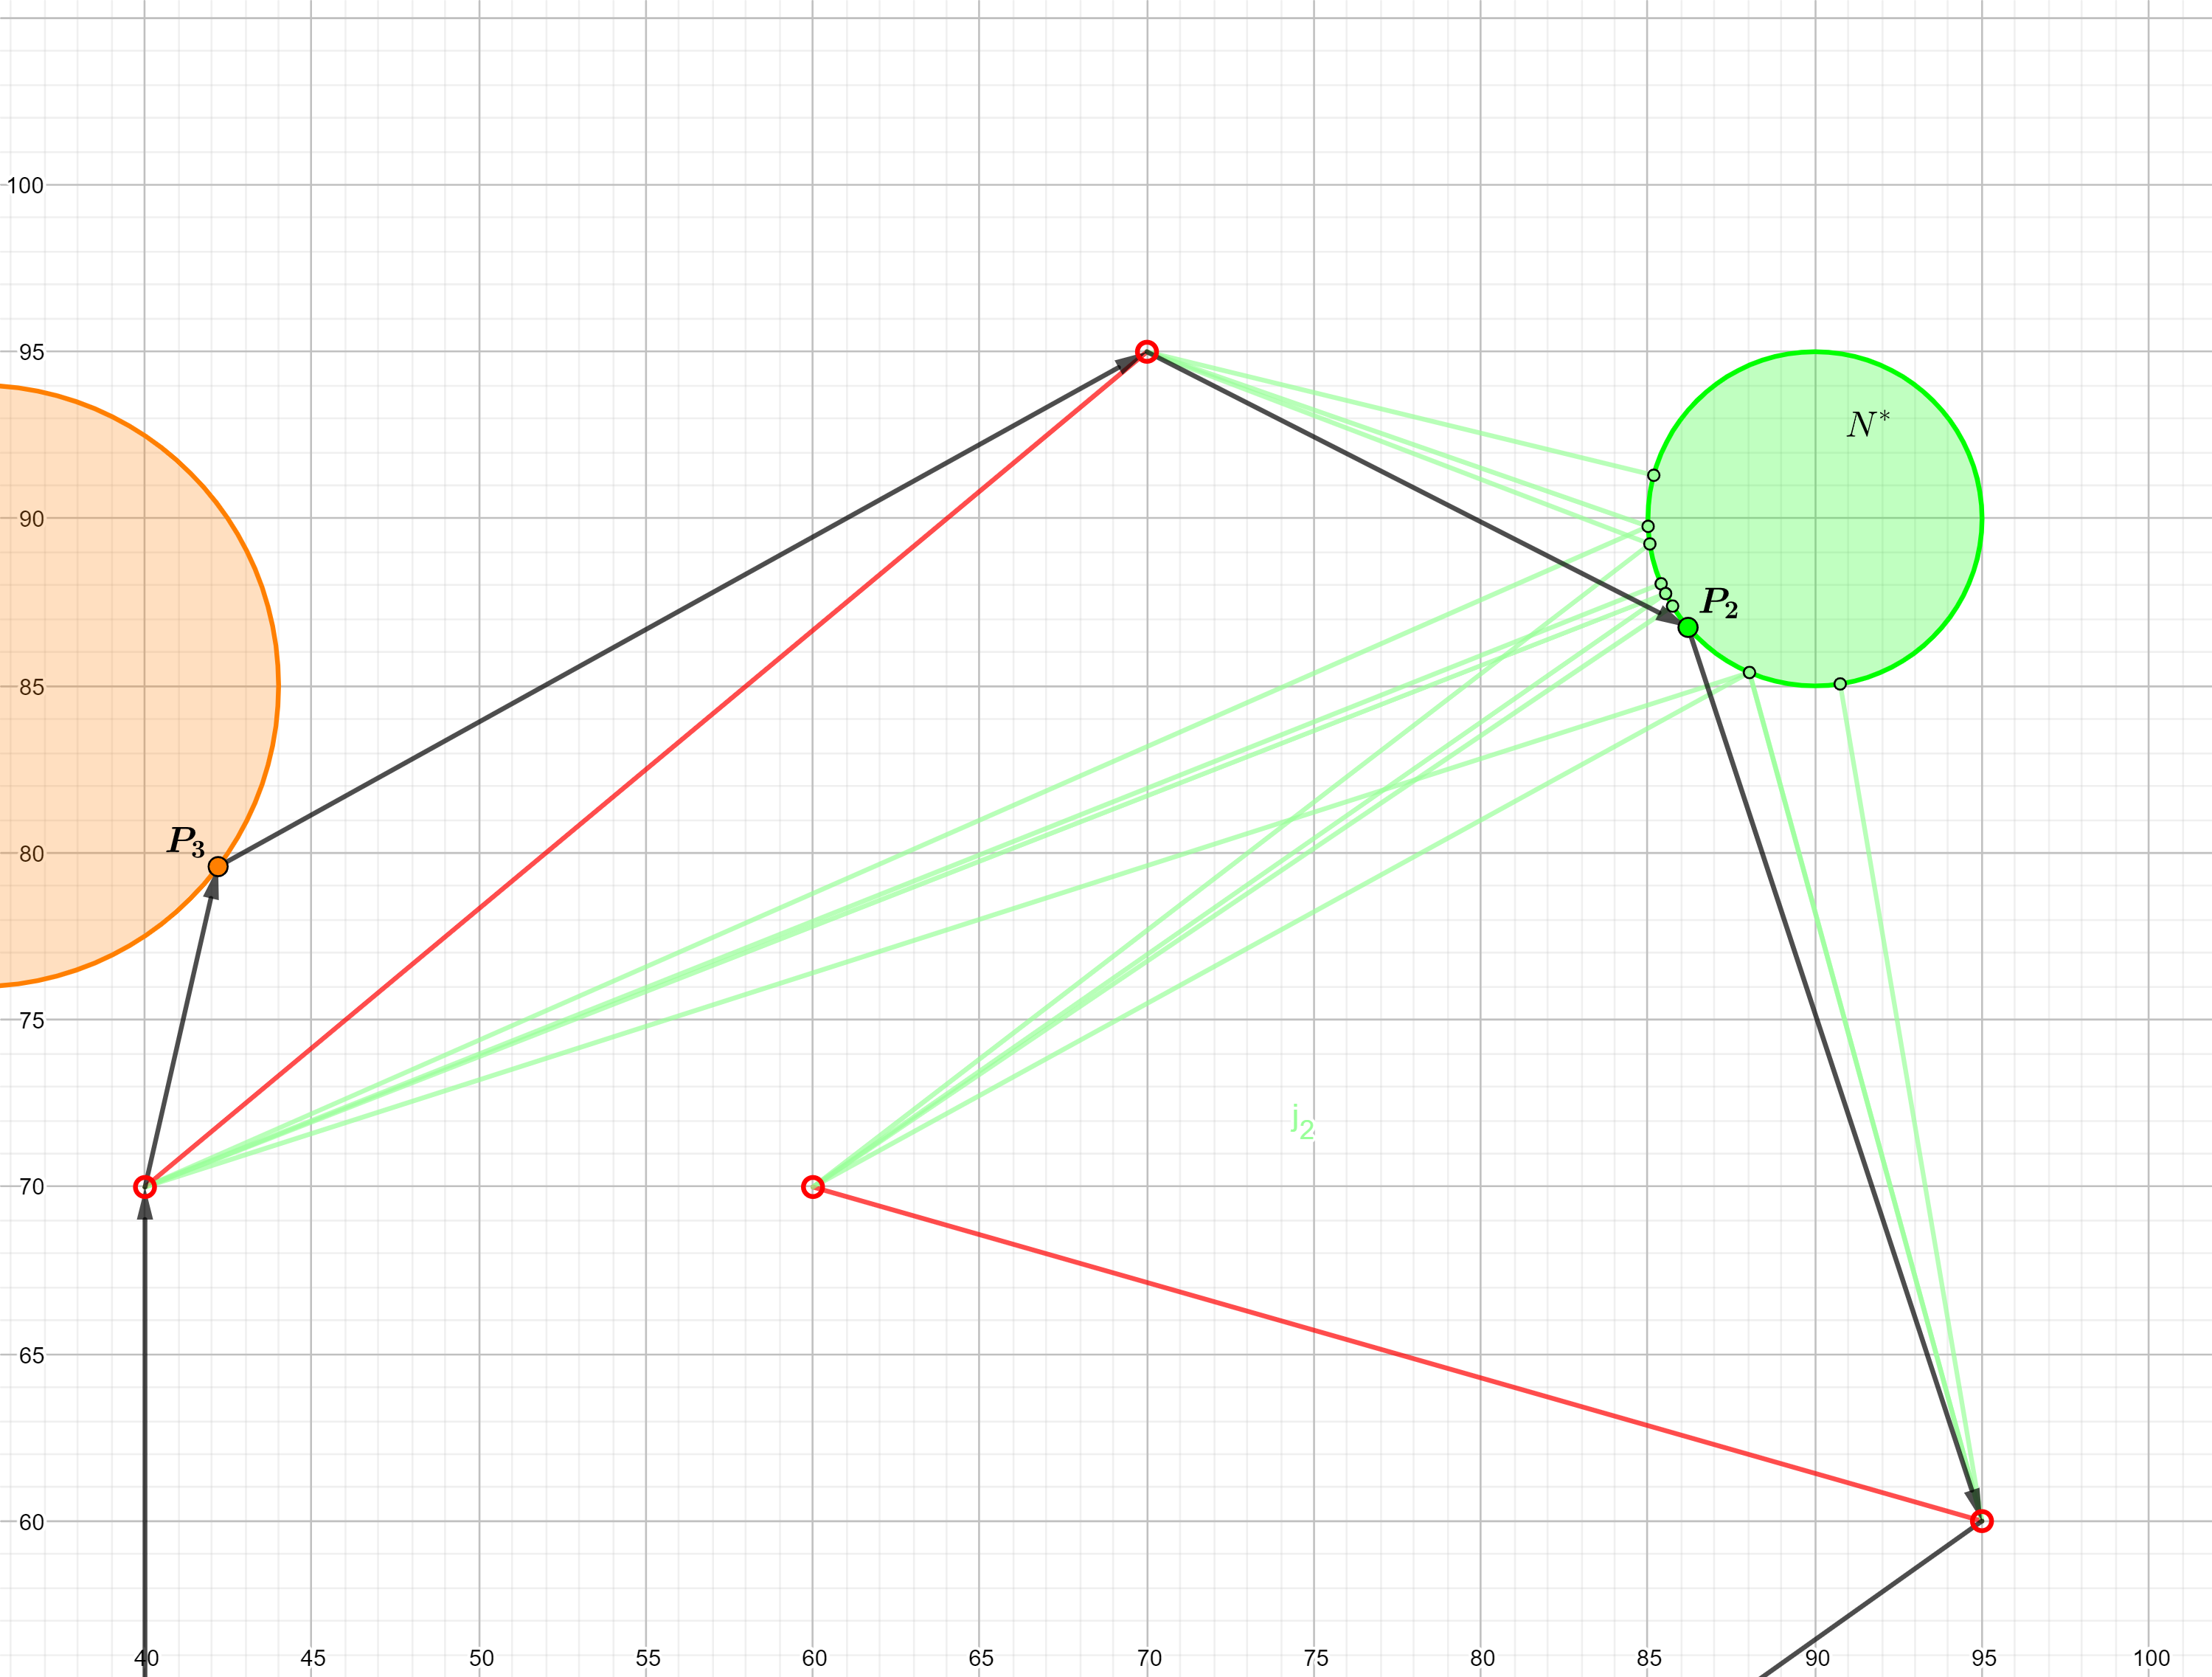
\includegraphics[width=0.8\linewidth]{dominating_sets_1_htspn}
		
		\end{figure}
	\end{frame}
	
	\begin{frame}{Reformulating the \KMPHN}
		\begin{figure}
			
			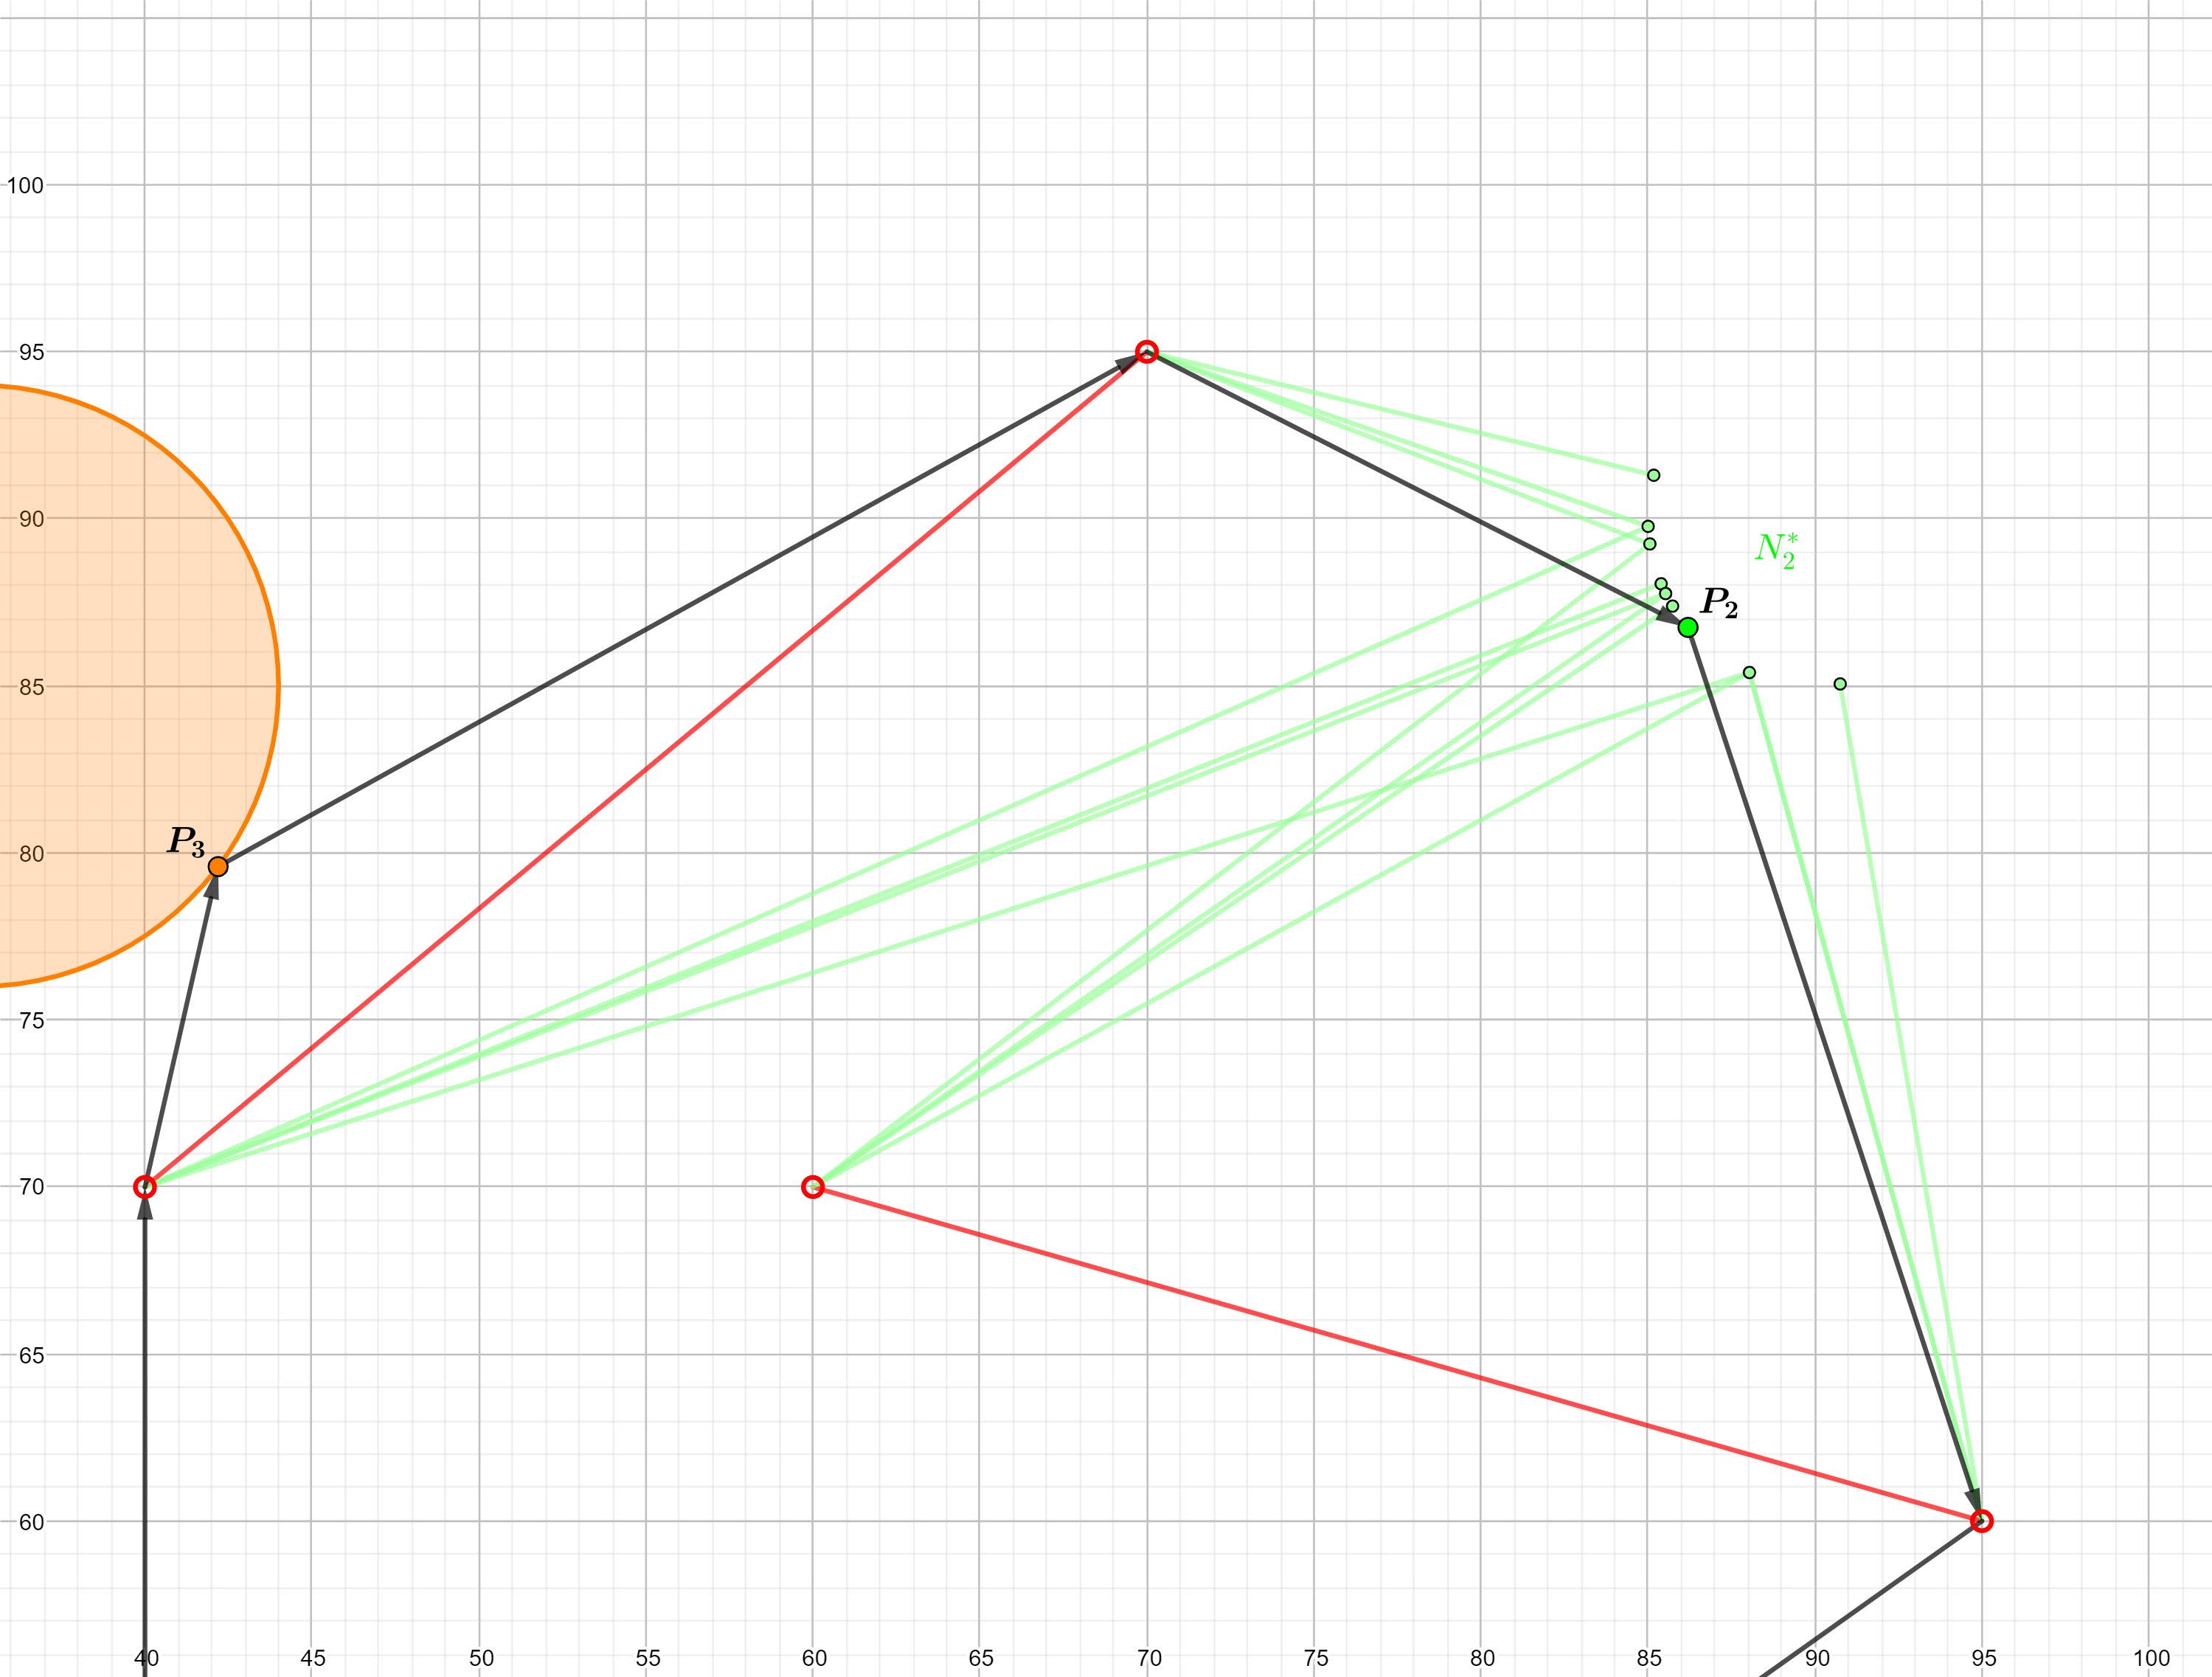
\includegraphics[width=0.8\linewidth]{dominating_sets_2_htspn}
			
		\end{figure}
	\end{frame}

	\begin{frame}{Solution of the Example}
		\begin{figure}
			\centering
			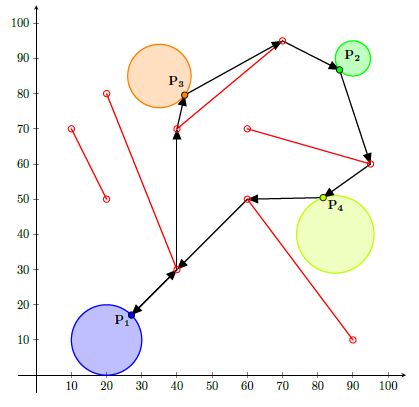
\includegraphics[width=0.6\linewidth]{solution_hidden_htspn}
			\caption{Solution for the TSPHN}
		\end{figure}
	\end{frame}
	
	\subsection{Strengthening formulations}
	\begin{frame}{Preprocessing}
		\begin{figure}[h!]
			\centering
			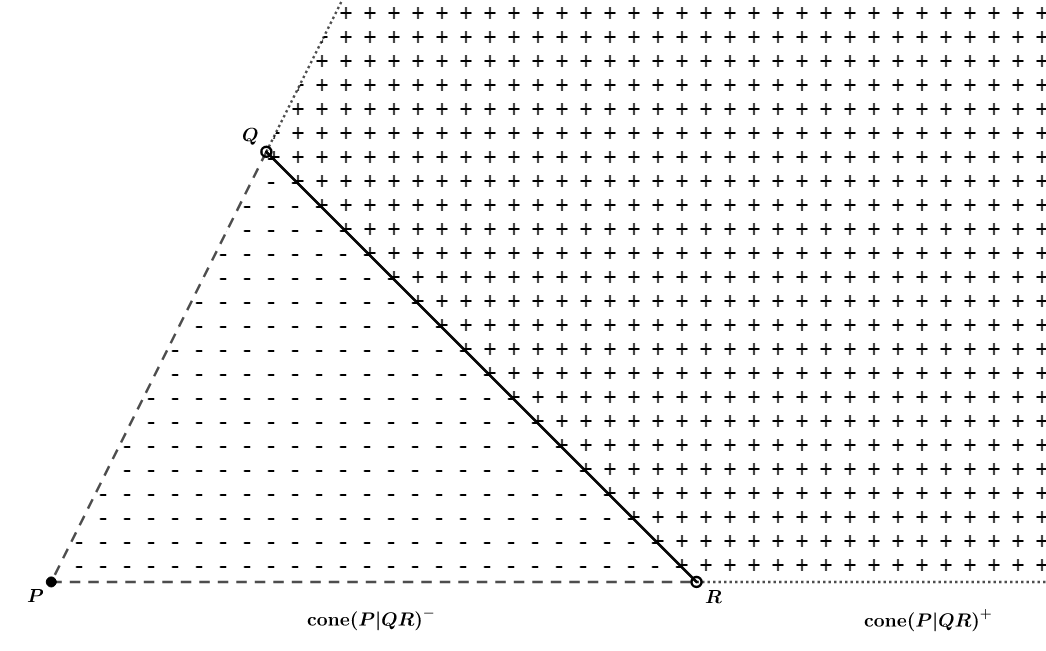
\includegraphics[width=0.75\linewidth]{cone_representation_htspn}
			\caption{Representation of the cone generated by the point $P$ and the line segment $\overline{QR}$.}
			\label{fig:cones}
		\end{figure}
	\end{frame}

	\begin{frame}{Preprocessing}

		\begin{prop}
			
			Let $B = \overline{P^1_BP^2_B}\in\mathcal B$ a barrier. If
			$$N\subset\bigcup_{B'\in\mathcal B}\normalfont{\text{cone}}(P^i_B| P^1_{B'}P^2_{B'})^+,$$
			then $(P^{}_N, P^i_B)\not\in \EN$.
			
			%Let $B'=\overline{P^1_{B'}P^2_{B'}}\in\mathcal B$ and $Q(B')$ the intersection point of the straight lines that join points of $N$ and $B'$ that lies outside of the convex hull generated by thse line segments. Let $\normalfont{\text{cone}}(\{\overrightarrow{Q(B')P^1_N},\overrightarrow{Q(B')P^2_N}\})$ the conical hull of these vectors. If
			%$$B\subset\bigcup_{B'\in\mathcal B}\normalfont{\text{cone}}(\{\overrightarrow{Q(B')P^1_N},\overrightarrow{Q(B')P^2_N}\}),$$
			%then $(P^{}_N, P^i_{B})\not\in \EN$, $i=1,2$.
		\end{prop}
		\begin{proof}
			If $P_N\in N$, then there exists a $B'\in\mathcal B$ such that 
			$P_N\in \normalfont{\text{cone}}(P^i_B|P^1_{B'}P^2_{B'})^+$. Therefore, $\overline{P^i_B P^{}_N}\cap B'\neq\emptyset$ and $(P^{}_N, P^i_B)\not\in \EN$.
		\end{proof}
	
	\end{frame}
	
	\begin{frame}
		\begin{figure}
			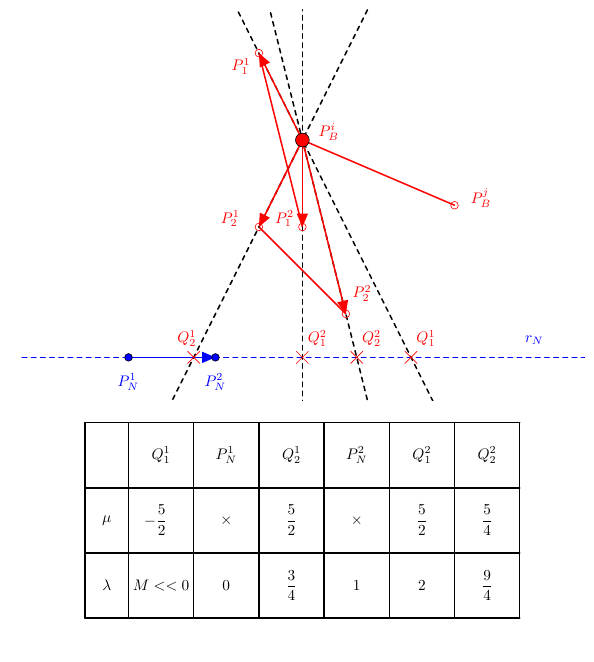
\includegraphics[width=0.6\linewidth]{example_preprocessing_htspn}
		\end{figure}
	\end{frame}

	\begin{frame}{Adjusting Big-Ms}
		Let $\overline{P^1_{B'}P^2_{B'}}=B'\in\B$ be a barrier, and $P_N\in N$. Let $\determinant{P_N}{P_{B'}^1}{P_{B'}^2}$ also be the determinant whose value must be bounded. Clearly, the solution of the following problem gives a lower bound of the determinant:
		\begin{equation*}\label{eq:L-Problem}
			\overline{L}=\min_{P_N=(x,y)\in N}F(x,y):=\determinant{P^{}_N}{P_{B'}^1}{P_{B'}^2}=\left|
			\begin{array}{cc}
				P^{1}_{B'_x}-x & P^{2}_{B'_x}-x \\
				P^{1}_{B'_y}-y & P^{2}_{B'_y}-y
			\end{array}
			\right|.
		\end{equation*}
		\begin{itemize}
			\item If $N$ is a segment:
				$$N=\{(x,y)\in\mathbb R^2:(x,y)=\mu P^1_{N}+(1-\mu)P^2_{N}, \; 0\leq\mu\leq1\}.$$
				The function achieves its minimum and maximum at the extreme points of $N$, i.e., $P_N^1$ and $P_N^2$.
		\end{itemize}
	\end{frame}

	\begin{frame}{Adjusting Big-Ms}
		\begin{itemize}
			\footnotesize
			\item If $N$ is a ellipse:
			$$N=\{(x,y)\in\mathbb R^2:ax^2+by^2+cxy+dx+ey+f\leq 0\}.$$
			Solving the quadratic system:
			$$
			\left\{\begin{array}{rl}
				\left[(2a, c)\cdot\overrightarrow{P^1_{B'}P^2_{B'}}\right]x+\left[(c, 2b)\cdot\overrightarrow{P^1_{B'}P^2_{B'}}\right]y+\left[(d, e)\cdot\overrightarrow{P^1_{B'}P^2_{B'}}\right]&=0,\\
				ax^2+by^2+cxy+dx+ey+f& =0,\\
			\end{array}\right.$$
			they arise two solutions $x^{\pm}$ and $y^{\pm}$ that are evaluated in the objective function to obtain the lowest and highest value, respectively, according to $\LS{P_N^{}}{P_{B'}^1}{P_{B'}^2}$ and $\US{P_N^{}}{P_{B'}^1}{P_{B'}^2}$, respectively.
		\end{itemize}
	\end{frame}

	\begin{frame}{Variable fixing}
		\footnotesize
		When a neighbourhood $N$ is in the half-space generated by a barrier $B$, the sign of the determinant $\determinant{P_N}{P_B^1}{P_B^2}$ does not change for any point $P_N\in N$.
		
		\begin{figure}
			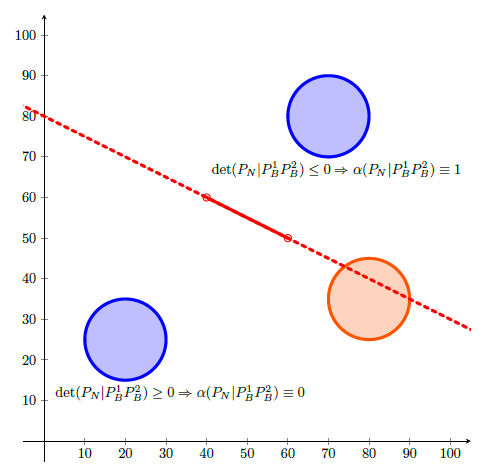
\includegraphics[width = 0.5\linewidth]{variable_fixing_htspn}
		\end{figure}
		Therefore, a relevant number of variables $\alpha$ (hence $\beta$, $\gamma$, $\delta$ and $\varepsilon$) that model the sign of this determinant can be fixed `a priori'.
	
	\end{frame}
	
	\subsection{Computational Experiments}
	
	\begin{frame}{Data Generation}
		Assumptions \textbf{A1}-\textbf{A4} stated before are assumed to create the instances of experiments. In this case, w.l.o.g., the neighbourhoods generated are segments and circles. 
		
		The sketch of the procedure is: 
		
		\begin{enumerate}
			\item Random sampling of the points in a square.
			\item Generation of the bisectors that separate any pair of points.
			\item Creation of the circles by assuming \textbf{A4}.
		\end{enumerate}
	
		The line segments instances are generated by randomly selecting two diametrically opposite points in the boundary of the balls instances.
		
		\medskip
		
		To generate instances for \KMPN, it is only required to remove some bisectors for the instances generated before to ensure that it is possible to go directly from one to another neighbourhood.
		
	\end{frame}

	\begin{frame}{Configuration of the experiments}
		Formulations were coded in Python 3.9.2 and solved in Gurobi 9.1.2 on an AMD® Epyc 7402p 8-core processor. A time limit of 1 hour was set for the solver procedure.
		
		\begin{itemize}
			\item Five instances of randomly-sized neighbourhoods $|\mathcal N|\in\{5, 10, 20, 30, 50, 60, 65, 70, 75, 80, 100\}$ in $R=[0,100]\times[0, 100]$
			\item Solving \KMPN \ and \KMPHN.
			\item Considering strengthening.
		\end{itemize}

	\end{frame}

%	\begin{frame}{Experimental Results (1)}
%	% Table generated by Excel2LaTeX from sheet 'Sheet1'
%	\begin{table}[htbp]
%		\centering
%		\caption{Table of computational results}
%		\resizebox{\linewidth}{!}{
%			\begin{tabular}{cccc|ccccc|ccccc|}
%			&   &   & \multicolumn{1}{c}{} & \multicolumn{5}{c}{\boldsymbol{$Circles$}} & \multicolumn{5}{c}{\boldsymbol{$Segments$}} \\
%			\boldsymbol{$|\mathcal N|$} & \boldsymbol{$A_4$} & \boldsymbol{$Strengthening$} & \boldsymbol{$|\mathcal B|$} & \boldsymbol{$\#Found$} & \boldsymbol{$Gap$} & \boldsymbol{$Time_{model}$} & \boldsymbol{$Time_{prepro}$} & \boldsymbol{$Time_{total}$} & \boldsymbol{$\#Found$} & \boldsymbol{$Gap$} & \boldsymbol{$Time_{model}$} & \boldsymbol{$Time_{prepro}$} & \boldsymbol{$Time_{total}$} \bigstrut[b]\\
%			\hline
%			\multirow{4}[4]{*}{5} & \multirow{2}[2]{*}{no} & no & 4.8 & 5 & 0 & 157.24 & 0.29 & 157.53 & 5 & 0 & 42.59 & 0.91 & 43.5 \bigstrut[t]\\
%			&   & yes & 4.8 & 5 & 0 & 1.24 & 0.44 & 1.68 & 5 & 0 & 0.42 & 1.47 & 1.89 \bigstrut[b]\\
%			\cline{2-14}      & \multirow{2}[2]{*}{yes} & no & 10.4 & 5 & 0.1 & 819.98 & 1.3 & 821.28 & 5 & 0 & 22.03 & 1.58 & 23.61 \bigstrut[t]\\
%			&   & yes & 10.4 & 5 & 0 & 0.61 & 1.16 & 1.77 & 5 & 0 & 0.38 & 1.57 & 1.95 \bigstrut[b]\\
%			\hline
%			\multirow{4}[4]{*}{10} & \multirow{2}[2]{*}{no} & no & 9.2 & 5 & 0.17 & 2193.53 & 2.09 & 2195.62 & 5 & 0.42 & 2884.22 & 6.6 & 2890.82 \bigstrut[t]\\
%			&   & yes & 9.2 & 5 & 0 & 9.1 & 2.58 & 11.68 & 5 & 0 & 1.69 & 9.61 & 11.3 \bigstrut[b]\\
%			\cline{2-14}      & \multirow{2}[2]{*}{yes} & no & 19.2 & 5 & 0.17 & 933.67 & 9.59 & 943.26 & 5 & 0.3 & 1448.73 & 11.8 & 1460.53 \bigstrut[t]\\
%			&   & yes & 19.2 & 5 & 0 & 2.56 & 6.36 & 8.92 & 5 & 0 & 1.53 & 9.24 & 10.77 \bigstrut[b]\\
%			\hline
%			\multirow{4}[4]{*}{20} & \multirow{2}[2]{*}{no} & no & 17.6 & 5 & 0.17 & 3600 & 16.15 & 3616.15 & 5 & 0.2 & 3600 & 50.93 & 3650.93 \bigstrut[t]\\
%			&   & yes & 17.6 & 5 & 0 & 68.67 & 17.43 & 86.1 & 5 & 0 & 11.66 & 74.89 & 86.55 \bigstrut[b]\\
%			\cline{2-14}      & \multirow{2}[2]{*}{yes} & no & 35.8 & 5 & 0.21 & 2349.26 & 87.7 & 2436.96 & 5 & 0 & 145.06 & 111.34 & 256.4 \bigstrut[t]\\
%			&   & yes & 35.8 & 5 & 0 & 42.45 & 43.49 & 85.94 & 5 & 0 & 8.05 & 64.01 & 72.06 \bigstrut[b]\\
%			\hline
%			\multirow{4}[4]{*}{30} & \multirow{2}[2]{*}{no} & no & 28 & 4 & 0.5 & 3600 & 75.15 & 3675.15 & 5 & 0.4 & 3600 & 201.05 & 3801.05 \bigstrut[t]\\
%			&   & yes & 28 & 5 & 0 & 2034.53 & 65.23 & 2099.76 & 5 & 0 & 54.35 & 246.96 & 301.31 \bigstrut[b]\\
%			\cline{2-14}      & \multirow{2}[2]{*}{yes} & no & 56.4 & 5 & 0.23 & 3027.02 & 512.03 & 3539.05 & 5 & 0.18 & 1039.08 & 672.46 & 1711.54 \bigstrut[t]\\
%			&   & yes & 56.4 & 5 & 0 & 147.98 & 179.95 & 327.93 & 5 & 0 & 96.72 & 270.56 & 367.28 \bigstrut[b]\\
%			\hline
%			\multirow{4}[4]{*}{50} & \multirow{2}[2]{*}{no} & no & 44.2 & 3 & 0.87 & 3600 & 364.75 & 3964.75 & 4 & 0.3 & 3600 & 960.53 & 4560.53 \bigstrut[t]\\
%			&   & yes & 44.2 & 3 & 0 & 2485.76 & 297.99 & 2783.75 & 5 & 0 & 311.49 & 1043.15 & 1354.64 \bigstrut[b]\\
%			\cline{2-14}      & \multirow{2}[2]{*}{yes} & no & 89 & 5 & 0.37 & 3600 & 4650.3 & 8250.3 & 5 & 0 & 1445.39 & 4654.95 & 6100.34 \bigstrut[t]\\
%			&   & yes & 89 & 5 & 0.1 & 3600 & 1213.85 & 4813.85 & 5 & 0 & 353.17 & 1292.12 & 1645.29 \bigstrut[b]\\
%			\hline
%		\end{tabular}}%
%	\label{table:results}%
%	\end{table}%	
%	
%	
%	
%\end{frame}

	\begin{frame}{Experimental Results (1)}
	% Table generated by Excel2LaTeX from sheet 'Sheet1'
	\begin{table}[htbp]
		\centering
		\caption{Computational results}
		\resizebox{\linewidth}{!}{
			\begin{tabular}{cccc|ccccc|ccccc|}
				&   &   & \multicolumn{1}{c}{} & \multicolumn{5}{c}{\boldsymbol{$Circles$}} & \multicolumn{5}{c}{\boldsymbol{$Segments$}} \\
				\boldsymbol{$|\mathcal N|$} & \boldsymbol{$A_4$} & \boldsymbol{$Strengthening$} & \boldsymbol{$|\mathcal B|$} & \boldsymbol{$\#Found$} & \boldsymbol{$Gap$} & \boldsymbol{$Time_{model}$} & \boldsymbol{$Time_{prepro}$} & \boldsymbol{$Time_{total}$} & \boldsymbol{$\#Found$} & \boldsymbol{$Gap$} & \boldsymbol{$Time_{model}$} & \boldsymbol{$Time_{prepro}$} & \boldsymbol{$Time_{total}$} \bigstrut[b]\\
				\hline
				\multirow{4}[4]{*}{5} & \multirow{2}[2]{*}{no} & no & 4.8 & 5 & 0 & 157.24 & 0.29 & 157.53 & 5 & 0 & 42.59 & 0.91 & 43.5 \bigstrut[t]\\
				&   & yes & 4.8 & 5 & 0 & 1.24 & 0.44 & 1.68 & 5 & 0 & 0.42 & 1.47 & 1.89 \bigstrut[b]\\
				\cline{2-14}      & \multirow{2}[2]{*}{yes} & no & 10.4 & 5 & 0.1 & 819.98 & 1.3 & 821.28 & 5 & 0 & 22.03 & 1.58 & 23.61 \bigstrut[t]\\
				&   & yes & 10.4 & 5 & 0 & 0.61 & 1.16 & 1.77 & 5 & 0 & 0.38 & 1.57 & 1.95 \bigstrut[b]\\
				\hline
				\multirow{4}[4]{*}{10} & \multirow{2}[2]{*}{no} & no & 9.2 & 5 & 0.17 & 2193.53 & 2.09 & 2195.62 & 5 & 0.42 & 2884.22 & 6.6 & 2890.82 \bigstrut[t]\\
				&   & yes & 9.2 & 5 & 0 & 9.1 & 2.58 & 11.68 & 5 & 0 & 1.69 & 9.61 & 11.3 \bigstrut[b]\\
				\cline{2-14}      & \multirow{2}[2]{*}{yes} & no & 19.2 & 5 & 0.17 & 933.67 & 9.59 & 943.26 & 5 & 0.3 & 1448.73 & 11.8 & 1460.53 \bigstrut[t]\\
				&   & yes & 19.2 & 5 & 0 & 2.56 & 6.36 & 8.92 & 5 & 0 & 1.53 & 9.24 & 10.77 \bigstrut[b]\\
				\hline
				\multirow{4}[4]{*}{20} & \multirow{2}[2]{*}{no} & no & 17.6 & 5 & 0.17 & 3600 & 16.15 & 3616.15 & 5 & 0.2 & 3600 & 50.93 & 3650.93 \bigstrut[t]\\
				&   & yes & 17.6 & 5 & 0 & 68.67 & 17.43 & 86.1 & 5 & 0 & 11.66 & 74.89 & 86.55 \bigstrut[b]\\
				\cline{2-14}      & \multirow{2}[2]{*}{yes} & no & 35.8 & 5 & 0.21 & 2349.26 & 87.7 & 2436.96 & 5 & 0 & 145.06 & 111.34 & 256.4 \bigstrut[t]\\
				&   & yes & 35.8 & 5 & 0 & 42.45 & 43.49 & 85.94 & 5 & 0 & 8.05 & 64.01 & 72.06 \bigstrut[b]\\
				\hline
				\multirow{4}[4]{*}{30} & \multirow{2}[2]{*}{no} & no & 28 & 4 & 0.5 & 3600 & 75.15 & 3675.15 & 5 & 0.4 & 3600 & 201.05 & 3801.05 \bigstrut[t]\\
				&   & yes & 28 & 5 & 0 & 2034.53 & 65.23 & 2099.76 & 5 & 0 & 54.35 & 246.96 & 301.31 \bigstrut[b]\\
				\cline{2-14}      & \multirow{2}[2]{*}{yes} & no & 56.4 & 5 & 0.23 & 3027.02 & 512.03 & 3539.05 & 5 & 0.18 & 1039.08 & 672.46 & 1711.54 \bigstrut[t]\\
				&   & yes & 56.4 & 5 & 0 & 147.98 & 179.95 & 327.93 & 5 & 0 & 96.72 & 270.56 & 367.28 \bigstrut[b]\\
				\hline
				\multirow{4}[4]{*}{50} & \multirow{2}[2]{*}{no} & no & 44.2 & 3 & 0.87 & 3600 & 364.75 & 3964.75 & 4 & 0.3 & 3600 & 960.53 & 4560.53 \bigstrut[t]\\
				&   & yes & 44.2 & 3 & 0 & 2485.76 & 297.99 & 2783.75 & 5 & 0 & 311.49 & 1043.15 & 1354.64 \bigstrut[b]\\
				\cline{2-14}      & \multirow{2}[2]{*}{yes} & no & 89 & 5 & 0.37 & 3600 & 4650.3 & 8250.3 & 5 & 0 & 1445.39 & 4654.95 & 6100.34 \bigstrut[t]\\
				&   & yes & 89 & 5 & 0.1 & 3600 & 1213.85 & 4813.85 & 5 & 0 & 353.17 & 1292.12 & 1645.29 \bigstrut[b]\\
				\hline
		\end{tabular}}%
		\label{table:results}%
	\end{table}%	
	
	\end{frame}

	\begin{frame}{Experimental Results (2)}
	\begin{table}[htbp]
	\centering
	\caption{Computational results}
	\resizebox{\linewidth}{!}{
		\begin{tabular}{cccc|ccccc|ccccc|}
			&   &   & \multicolumn{1}{c}{} & \multicolumn{5}{c}{\boldsymbol{$Circles$}} & \multicolumn{5}{c}{\boldsymbol{$Segments$}} \\
			\boldsymbol{$|\mathcal N|$} & \boldsymbol{$A_4$} & \boldsymbol{$Strengthening$} & \boldsymbol{$|\mathcal B|$} & \boldsymbol{$\#Found$} & \boldsymbol{$Gap$} & \boldsymbol{$Time_{model}$} & \boldsymbol{$Time_{prepro}$} & \boldsymbol{$Time_{total}$} & \boldsymbol{$\#Found$} & \boldsymbol{$Gap$} & \boldsymbol{$Time_{model}$} & \boldsymbol{$Time_{prepro}$} & \boldsymbol{$Time_{total}$} \bigstrut[b]\\
			\hline
			\multirow{4}[4]{*}{60} & \multirow{2}[2]{*}{no} & no & 50.2 & 0 & - & - & - & - & 5 & 0.53 & 3600 & 1213.08 & 4813.08 \bigstrut[t]\\
			&   & yes & 50.2 & 3 & 0.22 & 3600 & 538.11 & 4138.11 & 5 & 0 & 1384.92 & 1103.43 & 2488.35 \bigstrut[b]\\
			\cline{2-14}      & \multirow{2}[2]{*}{yes} & no & 100.8 & 5 & 0.15 & 3600 & 8688.65 & 12288.65 & 5 & 0 & 1671.85 & 8726.63 & 10398.48 \bigstrut[t]\\
			&   & yes & 100.8 & 5 & 0.13 & 3600 & 2179.26 & 5779.26 & 5 & 0.01 & 2903.27 & 2339.58 & 5242.85 \bigstrut[b]\\
			\hline
			\multirow{4}[4]{*}{65} & \multirow{2}[2]{*}{no} & no & 52.8 & 0 & - & - & - & - & 4 & 0.75 & 3600 & 1561.46 & 5161.46 \bigstrut[t]\\
			&   & yes & 52.8 & 2 & 0.35 & 3600 & 671.07 & 4271.07 & 5 & 0.02 & 3249.12 & 1343.12 & 4592.24 \bigstrut[b]\\
			\cline{2-14}      & \multirow{2}[2]{*}{yes} & no & 106 & 5 & 0.13 & 3600 & 11250.62 & 14850.62 & 5 & 0 & 1381.66 & 11269.25 & 12650.91 \bigstrut[t]\\
			&   & yes & 106 & 5 & 0.17 & 3600 & 2843.48 & 6443.48 & 5 & 0.01 & 2877.66 & 3003.47 & 5881.13 \bigstrut[b]\\
			\hline
			\multirow{4}[4]{*}{70} & \multirow{2}[2]{*}{no} & no & 57.6 & 0 & - & - & - & - & 4 & 0.85 & 3600 & 1977.3 & 5577.3 \bigstrut[t]\\
			&   & yes & 57.6 & 3 & 0.12 & 3600 & 898.99 & 4498.99 & 5 & 0.04 & 3211.2 & 1754.51 & 4965.71 \bigstrut[b]\\
			\cline{2-14}      & \multirow{2}[2]{*}{yes} & no & 115.6 & 5 & 0.29 & 3600 & 17366.28 & 20966.28 & 5 & 0.04 & 2853.58 & 17433.28 & 20286.86 \bigstrut[t]\\
			&   & yes & 115.6 & 5 & 0.32 & 3600 & 4106.95 & 7706.95 & 5 & 0.02 & 3203.33 & 4311.14 & 7514.47 \bigstrut[b]\\
			\hline
			\multirow{4}[4]{*}{75} & \multirow{2}[2]{*}{no} & no & 63.2 & 0 & - & - & - & - & 3 & 0.74 & 3600 & 2976.6 & 6576.6 \bigstrut[t]\\
			&   & yes & 63.2 & 0 & - & - & - & - & 5 & 0.24 & 3283.37 & 242407 & 5707,44 \bigstrut[b]\\
			\cline{2-14}      & \multirow{2}[2]{*}{yes} & no & 126.8 & 4 & 0.24 & 3600 & 26363.48 & 29963.48 & 5 & 0.01 & 1903.99 & 26153.87 & 28057.86 \bigstrut[t]\\
			&   & yes & 126.8 & 3 & 0.23 & 3600 & 5382.14 & 8982.14 & 5 & 0.02 & 2458.75 & 6140.02 & 8598.77 \bigstrut[b]\\
			\hline
			\multirow{4}[4]{*}{80} & \multirow{2}[2]{*}{no} & no & 64 & 0 & - & - & - & - & 1 & 0.83 & 3600 & 4205.41 & 7805.41 \bigstrut[t]\\
			&   & yes & 64 & 0 & - & - & - & - & 5 & 0 & 1775.16 & 2858.51 & 4633.67 \bigstrut[b]\\
			\cline{2-14}      & \multirow{2}[2]{*}{yes} & no & 128.6 & 0 & - & - & - & - & 5 & 0.11 & 3471.06 & 29073.69 & 32544.75 \bigstrut[t]\\
			&   & yes & 128.6 & 0 & - & - & - & - & 5 & 0 & 2701.21 & 7031.87 & 9733.08 \bigstrut[b]\\
			\hline
			\multirow{4}[4]{*}{100} & \multirow{2}[2]{*}{no} & no & 81.6 & 0 & - & - & - & - & 0 & - & - & - & - \bigstrut[t]\\
			&   & yes & 81.6 & 0 & - & - & - & - & 4 & 0 & 1761.08 & 6620.09 & 8381.17 \bigstrut[b]\\
			\cline{2-14}      & \multirow{2}[2]{*}{yes} & no & 163.2 & 0 & - & - & - & - & 5 & 0.48 & 3600 & 91153.55 & 94753.55 \bigstrut[t]\\
			&   & yes & 163.2 & 0 & - & - & - & - & 5 & 0 & 2720.76 & 19429.1 & 22149.86 \bigstrut[b]\\
			\hline
			\end{tabular}}%
			\label{table:results}%
		\end{table}%


		
	\end{frame}

	\begin{frame}{Further research}
		\begin{itemize}
			\item Study computationally non-disjoint neighbourhoods.
			\item Design some matheuristics to deal with larger instances.
			\item Consider non-convex neighbourhoods and/or nonlinear barriers.
			\item Propose alternative formulations that reduce the size of the problem.
			\item Extend to the third dimensional case.
			\item Study classical problems by including barriers.
		\end{itemize}
	\end{frame}

	\begin{frame}{Acknowledgements}
		This research has been partially supported by Spanish Ministry of Education and Science/FEDER grant number  MTM2016-74983-C02-(01-02), and projects FEDER-US-1256951, Junta de Andaluc\'ia P18-FR-1422, CEI-3-FQM331 and  \textit{NetmeetData}: Ayudas Fundaci\'on BBVA a equipos de investigaci\'on cient\'ifica 2019.
	\end{frame}
	
	\begin{frame}
		\bigskip
		\begin{figure}
			\centering
			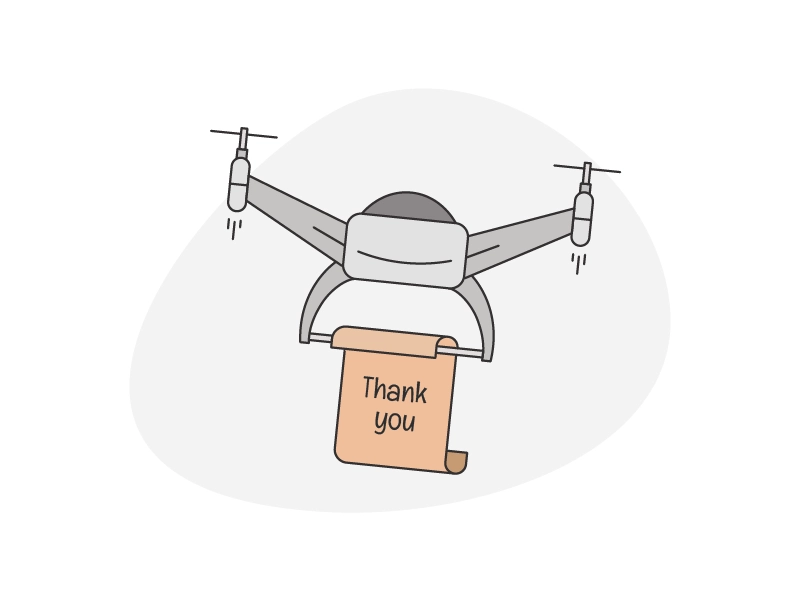
\includegraphics[width=0.7\linewidth]{thank}
			\label{fig:thank}
		\end{figure}
	\end{frame}
	
\end{document}